\def\ReportNumber{4}
\def\ReportName{Coupled magneto-thermal analysis}
\documentclass[11pt,a4paper]{article}
\usepackage[T1]{fontenc}
\usepackage[utf8]{inputenc}
\usepackage{newtxtext,newtxmath,microtype}
\usepackage[margin=21mm,headheight=14pt]{geometry}
\usepackage{booktabs,tabularx,array,amsmath,graphicx,float,caption}
\usepackage{xcolor,fancyhdr,lastpage,listings}
\usepackage[hidelinks]{hyperref}
\definecolor{accent}{HTML}{254C58}
% Original question wording: NMES Assignment 2026, Sections 1--3.
% Line-wrap hyphenation is removed; mathematical notation is typeset in LaTeX.
\usepackage{tcolorbox}
\newcommand{\assignmentquestion}[1]{%
  \begin{tcolorbox}[colback=accent!4,colframe=accent!65,
    boxrule=0.4pt,leftrule=2pt,arc=0pt,boxsep=0pt,
    left=7pt,right=7pt,top=5pt,bottom=5pt,
    before skip=0pt,after skip=8pt,fontupper=\small]
  \textbf{Assignment question.} #1
  \end{tcolorbox}%
}
\newcommand{\questionfiles}[1]{%
  \par\smallskip{\footnotesize\color{accent}
  \textbf{Files / results (relative to Source-code).} #1\par}\medskip
}
\newcommand{\QuestionOneOne}{%
Describe your cable: construction, dimensions, materials, rated voltage, rated
current (ampacity) and the laying conditions for which that rating is given
(burial depth, soil thermal resistivity, ambient temperature, arrangement).
Give a table of electromagnetic and thermal properties with a source for each value.}
\newcommand{\QuestionOneTwo}{%
Choose the environment consistently with the datasheet rating conditions,
and justify its properties.}
\newcommand{\QuestionOneThree}{%
State the sheath bonding you assume: single-point bonded (no net sheath current)
or solidly bonded (circulating sheath currents allowed), and how the armour
and pipe are connected. This choice strongly affects the losses in Section 3.}
\newcommand{\QuestionOneFour}{%
State the excitation you impose: phase-to-ground voltage and phase current,
as peak phasors, with the phase sequence (see the conventions in Appendix A).}
\newcommand{\QuestionTwoOne}{%
Define your computational domain, the equations solved and the boundary
conditions. Where do you truncate the domain, and why? Discuss the role of
the grounded screens: which regions actually influence the field in the insulation?}
\newcommand{\QuestionTwoTwo}{%
Can you simplify the geometry of your cable without degrading the precision
(e.g. disregard details in the geometrical description)? Quantify the effect
of each simplification.}
\newcommand{\QuestionTwoThree}{%
How do the results vary with the mesh refinement? Plot the maximum field in
the insulation and the capacitance versus the number of degrees of freedom,
and identify where local refinement is needed.}
\newcommand{\QuestionTwoFour}{%
Define the admissible field strength at the conductor screen and at the core
screen from the datasheet (or, if absent, from a cited reference).
Is the healthy cable within these limits?}
\newcommand{\QuestionTwoFive}{%
Add a defect to the insulation of your cable. State its nature (e.g. gas void,
water tree, protrusion of the semiconducting screen), its properties, size and
position, and discuss what a defect in a 2D cross-section represents in 3D.
Compare the field with and without defect along a radial cut.
Does the cable withstand the defect?}
\newcommand{\QuestionTwoSix}{%
Compute the resistive and displacement current densities in the cable.
Is current conservation satisfied? Which current dominates in each material, and why?}
\newcommand{\QuestionTwoSeven}{%
Compute the per-unit-length capacitance (\(\mu\mathrm{F/km}\)) and compare with
the analytical value (13) and with the datasheet. State the assumptions of the
analytical formula (in particular, how the semiconducting layers are treated).
Does the capacitance vary with frequency? Why (not)?}
\newcommand{\QuestionTwoEight}{%
Propose an improvement of the cable design with respect to the electric stress,
and support it quantitatively.}
\newcommand{\QuestionThreeOne}{%
Define your computational domain, the equations solved and the boundary conditions.
Where do you truncate the domain, and why? How do you impose the currents in the phase conductors?}
\newcommand{\QuestionThreeTwo}{%
\textbf{Conductor model.} Compare the skin depth in the conductor with its radius.
Model the phase conductors (a) as stranded conductors (imposed uniform current density)
and (b) as massive conductors (imposed net current, eddy currents allowed).
Which assumption is more realistic for your cable, and how does it affect the results?}
\newcommand{\QuestionThreeThree}{%
\textbf{Bonding.} Implement the bonding assumed in Q1.3 with global quantities
(net current and voltage per unit length in the sheaths, armour and pipe).
Explain why using only \(\mathbf j=-\mathrm i\omega\sigma\mathbf a\)
in these regions does not correspond to a well-defined bonding condition.}
\newcommand{\QuestionThreeFour}{%
Can you simplify the geometry without degrading the precision?
Are the simplifications of Section 2 still valid here?}
\newcommand{\QuestionThreeFive}{%
Check the mesh quality and refine where needed (element size compared with the
skin depth in each conducting region). How do losses, resistance and inductance
vary with the mesh refinement?}
\newcommand{\QuestionThreeSix}{%
Get the magnetic flux density (or induction) in and around your cable.}
\newcommand{\QuestionThreeSeven}{%
Get the current density in the conducting parts of your cable.}
\newcommand{\QuestionThreeEight}{%
Get the time-averaged Joule losses (kW/km) in each conducting part
(conductors, sheaths, armour, pipe, environment).}
\newcommand{\QuestionThreeNine}{%
Get the per-unit-length AC resistance (\(\Omega/\mathrm{km}\)), defined from
the total losses. Compare it with the DC resistance and with the datasheet.
Separate the contributions of skin/proximity effect and of sheath/armour losses.}
\newcommand{\QuestionThreeTen}{%
Get the per-unit-length inductance (mH/km). How do you define it for a
three-phase system? Does it vary with frequency? Compare with the datasheet.}
\newcommand{\QuestionThreeEleven}{%
Propose a design change that reduces the losses, and support it quantitatively.}

\pagestyle{fancy}\fancyhf{}
\fancyhead[L]{\small FE for Electromagnetic Fields -- Kutikuppala, Lefebure, Miseur}
\fancyhead[R]{\small NKT 33 kV, 185 + 50 mm\textsuperscript{2}}
\fancyfoot[L]{\small Section \ReportNumber\ -- \ReportName}
\fancyfoot[R]{\small\thepage\,/\,\pageref{LastPage}}
\renewcommand{\headrulewidth}{0.3pt}
\setlength{\parindent}{0pt}\setlength{\parskip}{5pt}
\setlength{\emergencystretch}{2em}
\setlength{\tabcolsep}{5pt}\renewcommand{\arraystretch}{1.13}
\captionsetup{font=small,labelfont=bf,skip=5pt}
\newcolumntype{Y}{>{\raggedright\arraybackslash}X}
\newcommand{\file}[1]{\href{../Source-code/#1}{\nolinkurl{#1}}}
\newcommand{\setupfile}[1]{\file{Cable-selection-and-model-setup/#1}}
\newcommand{\efile}{\file{Electrodynamic-analysis/cable.pro}}
\newcommand{\mfile}{\file{Magnetothermal-analysis/cable.pro}}
\newcommand{\runall}{\href{../run_all.sh}{\nolinkurl{run_all.sh}}}
\newcommand{\runE}{\texttt{getdp cable.pro -msh}\ \path{../Cable-selection-and-model-setup/cable.msh}\ \texttt{-solve Electrodynamics}}
\newcommand{\codeguide}[3]{\par\smallskip
 {\small\bfseries\color{accent}Code guide}\par\nobreak
 \begingroup\small\setlength{\tabcolsep}{0pt}
 \begin{tabularx}{\linewidth}{@{}p{14mm}Y@{}}
 \textbf{Files} & #1\\[2pt]
 \textbf{Run} & #2\\[2pt]
 \textbf{Check} & #3
 \end{tabularx}\par\endgroup\medskip}
\newcommand{\pending}{\textbf{Status: implementation still required.} }
\newcommand{\refurl}[2]{\href{#1}{#2}}
\lstset{basicstyle=\small\ttfamily,columns=fullflexible,keepspaces=true,
 showstringspaces=false,breaklines=true,upquote=true,
 backgroundcolor=\color{accent!4},frame=none,
 xleftmargin=5pt,xrightmargin=5pt,aboveskip=5pt,belowskip=5pt}
\hypersetup{pdftitle={Section \ReportNumber: \ReportName},
  pdfauthor={Kutikuppala Jaswanth, Lefebure Tiebert, Miseur Torre}}

\usepackage{pgfplots}\pgfplotsset{compat=1.18}
\graphicspath{{../../Slides/figures/}}
% Generated by Reports/collect_values.py. Do not edit.
\newcommand{\AmpLin}{386}
\newcommand{\Ampflat}{343}
\newcommand{\Ampflatsev}{352}
\newcommand{\Ampflatsevsp}{374}
\newcommand{\Ampflatsp}{351}
\newcommand{\Amptrefoil}{345}
\newcommand{\Amptrefoilsp}{350}
\newcommand{\AnaC}{0.197031}
\newcommand{\AnaCbare}{0.1834}
\newcommand{\AnaCthick}{0.181271}
\newcommand{\AnaDeltaAl}{11.96}
\newcommand{\AnaDeltaCu}{9.35}
\newcommand{\AnaDrop}{7}
\newcommand{\AnaEb}{5.14}
\newcommand{\AnaEi}{4.894}
\newcommand{\AnaEirms}{3.46}
\newcommand{\AnaEithick}{4.502}
\newcommand{\AnaEorms}{1.71}
\newcommand{\AnaEvoid}{6.20}
\newcommand{\AnaEzero}{4.34}
\newcommand{\AnaIch}{1.179}
\newcommand{\AnaJc}{\ensuremath{4.89\cdot10^{-12}}}
\newcommand{\AnaJd}{0.0340}
\newcommand{\AnaLgap}{0.4043}
\newcommand{\AnaLtouch}{0.4019}
\newcommand{\AnaRatio}{\ensuremath{1.44\cdot10^{-10}}}
\newcommand{\AnaWd}{0.022}
\newcommand{\AnaWdShare}{0.09}
\newcommand{\Bmax}{15.6}
\newcommand{\Bsingle}{13.4}
\newcommand{\Cdefect}{0.197000}
\newcommand{\Cdefectfine}{0.196999}
\newcommand{\Cffive}{0.197032}
\newcommand{\Cfhund}{0.197032}
\newcommand{\Cfthou}{0.197032}
\newcommand{\Cgap}{0.197032}
\newcommand{\Cgapcoarse}{0.197044}
\newcommand{\Cgapfine}{0.197031}
\newcommand{\CondShare}{94}
\newcommand{\ConvRate}{0.22}
\newcommand{\Cqdefect}{0.196937}
\newcommand{\Cqdefectfine}{0.196935}
\newcommand{\Cqffive}{0.197032}
\newcommand{\Cqfhund}{0.197032}
\newcommand{\Cqfthou}{0.197032}
\newcommand{\Cqgap}{0.197032}
\newcommand{\Cqgapcoarse}{0.197044}
\newcommand{\Cqgapfine}{0.197031}
\newcommand{\Cqthick}{0.181272}
\newcommand{\Cqtouching}{0.197032}
\newcommand{\Cthick}{0.181272}
\newcommand{\Ctouching}{0.197032}
\newcommand{\Dofsdefect}{65\,900}
\newcommand{\Dofsdefectfine}{265\,156}
\newcommand{\Dofsffive}{64\,884}
\newcommand{\Dofsfhund}{64\,884}
\newcommand{\Dofsfthou}{64\,884}
\newcommand{\Dofsgap}{64\,884}
\newcommand{\Dofsgapcoarse}{16\,100}
\newcommand{\Dofsgapfine}{261\,058}
\newcommand{\Dofsthick}{76\,210}
\newcommand{\Dofstouching}{64\,880}
\newcommand{\EddyFE}{0.9}
\newcommand{\Edefect}{6.29}
\newcommand{\Edefectfine}{6.30}
\newcommand{\Effive}{4.873}
\newcommand{\Efhund}{4.873}
\newcommand{\Efthou}{4.873}
\newcommand{\Egap}{4.873}
\newcommand{\Egapcoarse}{4.846}
\newcommand{\Egapfine}{4.885}
\newcommand{\Ethick}{4.474}
\newcommand{\Etouching}{4.872}
\newcommand{\Hrad}{5.2}
\newcommand{\Ibalance}{\ensuremath{4\cdot10^{-14}}}
\newcommand{\IchFE}{1.179}
\newcommand{\IecAmp}{351}
\newcommand{\IecIs}{56.8}
\newcommand{\IecLam}{5.52}
\newcommand{\IecLamHot}{3.6}
\newcommand{\IecPc}{60.55}
\newcommand{\IecPcHot}{76.8}
\newcommand{\IecPs}{3.34}
\newcommand{\IecPsHot}{2.76}
\newcommand{\IecPt}{63.89}
\newcommand{\IecRac}{0.1739}
\newcommand{\IecRacHot}{0.2164}
\newcommand{\IecRcond}{0.16475}
\newcommand{\IecRcondHot}{0.2089}
\newcommand{\IecRs}{0.3448}
\newcommand{\IecTfour}{2.236}
\newcommand{\IecTheta}{89.2}
\newcommand{\IecThetaS}{77}
\newcommand{\IecTone}{0.476}
\newcommand{\IecTthree}{0.104}
\newcommand{\IecU}{46.5}
\newcommand{\IecUs}{19.9}
\newcommand{\IecX}{0.0568}
\newcommand{\IecYp}{0.15}
\newcommand{\IecYs}{0.31}
\newcommand{\IecYsp}{0.46}
\newcommand{\Ioneflat}{341}
\newcommand{\Ioneflatsev}{353}
\newcommand{\Ioneflatsevsp}{381}
\newcommand{\Ioneflatsp}{351}
\newcommand{\Ionetrefoil}{344}
\newcommand{\Ionetrefoilsp}{350}
\newcommand{\IratioFE}{\ensuremath{1.44\cdot10^{-10}}}
\newcommand{\IsPeak}{79}
\newcommand{\IsSum}{0.15}
\newcommand{\Isbase}{55.5}
\newcommand{\Isbox}{55.9}
\newcommand{\Iscoarse}{54.9}
\newcommand{\Isfdc}{0.0}
\newcommand{\Isffive}{5.7}
\newcommand{\Isfhund}{267.6}
\newcommand{\Isfine}{55.8}
\newcommand{\Isflat}{60.9}
\newcommand{\IsflatIone}{60.0}
\newcommand{\Isflatsev}{95.4}
\newcommand{\IsflatsevIone}{95.9}
\newcommand{\Isflatsevsp}{0.0}
\newcommand{\IsflatsevspIone}{0.0}
\newcommand{\Isflatsp}{0.0}
\newcommand{\IsflatspIone}{0.0}
\newcommand{\Islin}{55.5}
\newcommand{\Isliniso}{55.5}
\newcommand{\Isnl}{45.4}
\newcommand{\Isnlcoarse}{45.0}
\newcommand{\Isnldomforty}{45.4}
\newcommand{\Isnldomten}{45.4}
\newcommand{\Isnlfine}{45.5}
\newcommand{\Isnlhfive}{45.2}
\newcommand{\Isnlhtwenty}{45.5}
\newcommand{\Isnliso}{45.6}
\newcommand{\Issingle}{0.0}
\newcommand{\Isstranded}{55.6}
\newcommand{\Isstrandedfhund}{268.1}
\newcommand{\Istouching}{54.9}
\newcommand{\Istrefoil}{45.4}
\newcommand{\IstrefoilIone}{45.0}
\newcommand{\Istrefoilsp}{0.0}
\newcommand{\IstrefoilspIone}{0.0}
\newcommand{\Javg}{2.88}
\newcommand{\JcFE}{\ensuremath{4.87\cdot10^{-12}}}
\newcommand{\JdFE}{0.0339}
\newcommand{\Jmax}{3.07}
\newcommand{\Jscreen}{1.6}
\newcommand{\LamFE}{6.1}
\newcommand{\Lbase}{0.3943}
\newcommand{\Lbox}{0.3955}
\newcommand{\Lcoarse}{0.3922}
\newcommand{\Lfdc}{0.4010}
\newcommand{\Lffive}{0.4010}
\newcommand{\Lfhund}{0.2616}
\newcommand{\Lfine}{0.3952}
\newcommand{\Lflat}{0.4331}
\newcommand{\LflatIone}{0.4328}
\newcommand{\Lflatsev}{0.5722}
\newcommand{\LflatsevIone}{0.5724}
\newcommand{\Lflatsevsp}{0.6061}
\newcommand{\LflatsevspIone}{0.6061}
\newcommand{\Lflatsp}{0.4437}
\newcommand{\LflatspIone}{0.4437}
\newcommand{\Llin}{0.3943}
\newcommand{\Lliniso}{0.3943}
\newcommand{\Lnl}{0.3965}
\newcommand{\Lnlcoarse}{0.3944}
\newcommand{\Lnldomforty}{0.3965}
\newcommand{\Lnldomten}{0.3965}
\newcommand{\Lnlfine}{0.3975}
\newcommand{\Lnlhfive}{0.3966}
\newcommand{\Lnlhtwenty}{0.3965}
\newcommand{\Lnliso}{0.3965}
\newcommand{\Lsingle}{0.4003}
\newcommand{\Lstranded}{0.3947}
\newcommand{\Lstrandedfhund}{0.2670}
\newcommand{\Lterm}{0.3945}
\newcommand{\Ltouching}{0.3923}
\newcommand{\Ltrefoil}{0.3965}
\newcommand{\LtrefoilIone}{0.3965}
\newcommand{\Ltrefoilsp}{0.4006}
\newcommand{\LtrefoilspIone}{0.4006}
\newcommand{\MDofsbase}{295\,294}
\newcommand{\MDofsbox}{297\,138}
\newcommand{\MDofscoarse}{75\,856}
\newcommand{\MDofsfdc}{295\,294}
\newcommand{\MDofsffive}{295\,294}
\newcommand{\MDofsfhund}{295\,294}
\newcommand{\MDofsfine}{1\,169\,120}
\newcommand{\MDofsflat}{243\,780}
\newcommand{\MDofsflatIone}{243\,780}
\newcommand{\MDofsflatsev}{253\,538}
\newcommand{\MDofsflatsevIone}{253\,538}
\newcommand{\MDofsflatsevsp}{253\,538}
\newcommand{\MDofsflatsevspIone}{253\,538}
\newcommand{\MDofsflatsp}{243\,780}
\newcommand{\MDofsflatspIone}{243\,780}
\newcommand{\MDofslin}{295\,294}
\newcommand{\MDofsliniso}{295\,294}
\newcommand{\MDofsnl}{295\,294}
\newcommand{\MDofsnlcoarse}{75\,856}
\newcommand{\MDofsnldomforty}{295\,294}
\newcommand{\MDofsnldomten}{295\,294}
\newcommand{\MDofsnlfine}{1\,169\,120}
\newcommand{\MDofsnlhfive}{295\,294}
\newcommand{\MDofsnlhtwenty}{295\,294}
\newcommand{\MDofsnliso}{295\,294}
\newcommand{\MDofssingle}{295\,294}
\newcommand{\MDofsstranded}{295\,288}
\newcommand{\MDofsstrandedfhund}{295\,288}
\newcommand{\MDofstouching}{292\,266}
\newcommand{\MDofstrefoil}{295\,294}
\newcommand{\MDofstrefoilIone}{295\,294}
\newcommand{\MDofstrefoilsp}{295\,294}
\newcommand{\MDofstrefoilspIone}{295\,294}
\newcommand{\MeshBadGap}{0}
\newcommand{\MeshBadTouch}{24}
\newcommand{\MeshQminGap}{0.575}
\newcommand{\MeshQminTouch}{0.020}
\newcommand{\MeshTriGap}{297\,943}
\newcommand{\MeshTriTouch}{294\,915}
\newcommand{\MeshXlpeGap}{22\,228}
\newcommand{\MeshXlpeTouch}{22\,222}
\newcommand{\Nitflat}{10}
\newcommand{\NitflatIone}{10}
\newcommand{\Nitflatsev}{9}
\newcommand{\NitflatsevIone}{9}
\newcommand{\Nitflatsevsp}{10}
\newcommand{\NitflatsevspIone}{11}
\newcommand{\Nitflatsp}{10}
\newcommand{\NitflatspIone}{10}
\newcommand{\Nitlin}{1}
\newcommand{\Nitliniso}{1}
\newcommand{\Nitnl}{10}
\newcommand{\Nitnlcoarse}{10}
\newcommand{\Nitnldomforty}{10}
\newcommand{\Nitnldomten}{10}
\newcommand{\Nitnlfine}{10}
\newcommand{\Nitnlhfive}{10}
\newcommand{\Nitnlhtwenty}{10}
\newcommand{\Nitnliso}{10}
\newcommand{\Nittrefoil}{10}
\newcommand{\NittrefoilIone}{10}
\newcommand{\Nittrefoilsp}{10}
\newcommand{\NittrefoilspIone}{10}
\newcommand{\NktL}{0.382}
\newcommand{\PcPhase}{20.18}
\newcommand{\Pcbase}{60.55}
\newcommand{\Pcbox}{60.55}
\newcommand{\Pccoarse}{60.58}
\newcommand{\Pcfdc}{60.28}
\newcommand{\Pcffive}{60.28}
\newcommand{\Pcfhund}{75.76}
\newcommand{\Pcfine}{60.54}
\newcommand{\Pcflat}{77.44}
\newcommand{\PcflatIone}{72.36}
\newcommand{\Pcflatsev}{76.02}
\newcommand{\PcflatsevIone}{77.69}
\newcommand{\Pcflatsevsp}{73.63}
\newcommand{\PcflatsevspIone}{91.14}
\newcommand{\Pcflatsp}{76.37}
\newcommand{\PcflatspIone}{77.04}
\newcommand{\PcircFE}{3.16}
\newcommand{\Pclin}{60.55}
\newcommand{\Pcliniso}{60.55}
\newcommand{\Pcnl}{77.58}
\newcommand{\Pcnlcoarse}{77.38}
\newcommand{\Pcnldomforty}{77.59}
\newcommand{\Pcnldomten}{77.51}
\newcommand{\Pcnlfine}{77.65}
\newcommand{\Pcnlhfive}{77.92}
\newcommand{\Pcnlhtwenty}{77.40}
\newcommand{\Pcnliso}{77.21}
\newcommand{\Pcsingle}{60.55}
\newcommand{\Pcstranded}{60.26}
\newcommand{\Pcstrandedfhund}{60.26}
\newcommand{\Pctouching}{60.55}
\newcommand{\Pctrefoil}{77.58}
\newcommand{\PctrefoilIone}{74.07}
\newcommand{\Pctrefoilsp}{76.94}
\newcommand{\PctrefoilspIone}{76.94}
\newcommand{\PdInception}{16}
\newcommand{\PhaseSym}{0.0004}
\newcommand{\Psbase}{3.68}
\newcommand{\Psbox}{3.74}
\newcommand{\Pscoarse}{3.59}
\newcommand{\Psfdc}{0.00}
\newcommand{\Psffive}{0.04}
\newcommand{\Psfhund}{81.84}
\newcommand{\Psfine}{3.72}
\newcommand{\Psflat}{5.01}
\newcommand{\PsflatIone}{4.81}
\newcommand{\Psflatsev}{12.34}
\newcommand{\PsflatsevIone}{12.51}
\newcommand{\Psflatsevsp}{0.05}
\newcommand{\PsflatsevspIone}{0.05}
\newcommand{\Psflatsp}{0.41}
\newcommand{\PsflatspIone}{0.41}
\newcommand{\Pslin}{3.68}
\newcommand{\Psliniso}{3.68}
\newcommand{\Psnl}{3.03}
\newcommand{\Psnlcoarse}{2.96}
\newcommand{\Psnldomforty}{3.03}
\newcommand{\Psnldomten}{3.03}
\newcommand{\Psnlfine}{3.06}
\newcommand{\Psnlhfive}{3.02}
\newcommand{\Psnlhtwenty}{3.04}
\newcommand{\Psnliso}{3.04}
\newcommand{\Pssingle}{0.52}
\newcommand{\Psstranded}{3.70}
\newcommand{\Psstrandedfhund}{83.03}
\newcommand{\Pstouching}{3.62}
\newcommand{\Pstrefoil}{3.03}
\newcommand{\PstrefoilIone}{2.95}
\newcommand{\Pstrefoilsp}{0.43}
\newcommand{\PstrefoilspIone}{0.43}
\newcommand{\Ptbase}{64.23}
\newcommand{\Ptbox}{64.30}
\newcommand{\Ptcoarse}{64.17}
\newcommand{\Ptfdc}{60.28}
\newcommand{\Ptffive}{60.32}
\newcommand{\Ptfhund}{157.60}
\newcommand{\Ptfine}{64.27}
\newcommand{\Ptflat}{82.45}
\newcommand{\PtflatIone}{77.17}
\newcommand{\Ptflatsev}{88.36}
\newcommand{\PtflatsevIone}{90.20}
\newcommand{\Ptflatsevsp}{73.68}
\newcommand{\PtflatsevspIone}{91.20}
\newcommand{\Ptflatsp}{76.77}
\newcommand{\PtflatspIone}{77.45}
\newcommand{\Ptlin}{64.23}
\newcommand{\Ptliniso}{64.23}
\newcommand{\Ptnl}{80.61}
\newcommand{\Ptnlcoarse}{80.33}
\newcommand{\Ptnldomforty}{80.62}
\newcommand{\Ptnldomten}{80.55}
\newcommand{\Ptnlfine}{80.71}
\newcommand{\Ptnlhfive}{80.94}
\newcommand{\Ptnlhtwenty}{80.43}
\newcommand{\Ptnliso}{80.25}
\newcommand{\Ptsingle}{61.07}
\newcommand{\Ptstranded}{63.96}
\newcommand{\Ptstrandedfhund}{143.29}
\newcommand{\Pttouching}{64.17}
\newcommand{\Pttrefoil}{80.61}
\newcommand{\PttrefoilIone}{77.02}
\newcommand{\Pttrefoilsp}{77.36}
\newcommand{\PttrefoilspIone}{77.36}
\newcommand{\QsFrac}{94.6}
\newcommand{\Racbase}{0.1748}
\newcommand{\Racbox}{0.1750}
\newcommand{\Raccoarse}{0.1746}
\newcommand{\Racfdc}{0.1640}
\newcommand{\Racffive}{0.1641}
\newcommand{\Racfhund}{0.4288}
\newcommand{\Racfine}{0.1749}
\newcommand{\Racflat}{0.2244}
\newcommand{\RacflatIone}{0.2214}
\newcommand{\Racflatsev}{0.2404}
\newcommand{\RacflatsevIone}{0.2413}
\newcommand{\Racflatsevsp}{0.2005}
\newcommand{\RacflatsevspIone}{0.2097}
\newcommand{\Racflatsp}{0.2089}
\newcommand{\RacflatspIone}{0.2093}
\newcommand{\Raclin}{0.1748}
\newcommand{\Racliniso}{0.1748}
\newcommand{\Racnl}{0.2193}
\newcommand{\Racnlcoarse}{0.2186}
\newcommand{\Racnldomforty}{0.2194}
\newcommand{\Racnldomten}{0.2192}
\newcommand{\Racnlfine}{0.2196}
\newcommand{\Racnlhfive}{0.2202}
\newcommand{\Racnlhtwenty}{0.2189}
\newcommand{\Racnliso}{0.2184}
\newcommand{\Racsingle}{0.1662}
\newcommand{\Racstranded}{0.1740}
\newcommand{\Racstrandedfhund}{0.3899}
\newcommand{\Ractouching}{0.1746}
\newcommand{\Ractrefoil}{0.2193}
\newcommand{\RactrefoilIone}{0.2172}
\newcommand{\Ractrefoilsp}{0.2105}
\newcommand{\RactrefoilspIone}{0.2105}
\newcommand{\Rcbase}{0.1648}
\newcommand{\Rcbox}{0.1648}
\newcommand{\Rccoarse}{0.1648}
\newcommand{\Rcfdc}{0.1640}
\newcommand{\Rcffive}{0.1640}
\newcommand{\Rcfhund}{0.2061}
\newcommand{\Rcfine}{0.1647}
\newcommand{\Rcflat}{0.2107}
\newcommand{\RcflatIone}{0.2076}
\newcommand{\Rcflatsev}{0.2069}
\newcommand{\RcflatsevIone}{0.2078}
\newcommand{\Rcflatsevsp}{0.2004}
\newcommand{\RcflatsevspIone}{0.2096}
\newcommand{\Rcflatsp}{0.2078}
\newcommand{\RcflatspIone}{0.2082}
\newcommand{\Rclin}{0.1648}
\newcommand{\Rcliniso}{0.1648}
\newcommand{\Rcnl}{0.2111}
\newcommand{\Rcnlcoarse}{0.2105}
\newcommand{\Rcnldomforty}{0.2111}
\newcommand{\Rcnldomten}{0.2109}
\newcommand{\Rcnlfine}{0.2113}
\newcommand{\Rcnlhfive}{0.2120}
\newcommand{\Rcnlhtwenty}{0.2106}
\newcommand{\Rcnliso}{0.2101}
\newcommand{\Rcsingle}{0.1648}
\newcommand{\Rcstranded}{0.1640}
\newcommand{\Rcstrandedfhund}{0.1640}
\newcommand{\Rctouching}{0.1648}
\newcommand{\Rctrefoil}{0.2111}
\newcommand{\RctrefoilIone}{0.2089}
\newcommand{\Rctrefoilsp}{0.2094}
\newcommand{\RctrefoilspIone}{0.2094}
\newcommand{\RhoHot}{28}
\newcommand{\ScreenFE}{6.1}
\newcommand{\SkinFE}{0.45}
\newcommand{\TDofsnl}{149\,003}
\newcommand{\TcA}{92.52}
\newcommand{\TcB}{92.74}
\newcommand{\TcC}{92.74}
\newcommand{\Tcflat}{94.1}
\newcommand{\TcflatIone}{89.0}
\newcommand{\Tcflatsev}{88.7}
\newcommand{\TcflatsevIone}{90.3}
\newcommand{\Tcflatsevsp}{78.4}
\newcommand{\TcflatsevspIone}{93.5}
\newcommand{\Tcflatsp}{89.5}
\newcommand{\TcflatspIone}{90.1}
\newcommand{\Tclin}{76.7}
\newcommand{\Tcliniso}{75.8}
\newcommand{\Tcnl}{92.7}
\newcommand{\Tcnlcoarse}{91.7}
\newcommand{\Tcnldomforty}{92.8}
\newcommand{\Tcnldomten}{92.5}
\newcommand{\Tcnlfine}{93.1}
\newcommand{\Tcnlhfive}{94.2}
\newcommand{\Tcnlhtwenty}{92.0}
\newcommand{\Tcnliso}{91.2}
\newcommand{\Tctrefoil}{92.7}
\newcommand{\TctrefoilIone}{89.3}
\newcommand{\Tctrefoilsp}{90.0}
\newcommand{\TctrefoilspIone}{90.0}
\newcommand{\Tsflat}{17.42}
\newcommand{\TsflatIone}{17.27}
\newcommand{\Tsflatsev}{17.58}
\newcommand{\TsflatsevIone}{17.63}
\newcommand{\Tsflatsevsp}{17.15}
\newcommand{\TsflatsevspIone}{17.66}
\newcommand{\Tsflatsp}{17.25}
\newcommand{\TsflatspIone}{17.27}
\newcommand{\Tslin}{16.89}
\newcommand{\Tsliniso}{15.00}
\newcommand{\Tsnl}{17.37}
\newcommand{\Tsnlcoarse}{17.36}
\newcommand{\Tsnldomforty}{17.37}
\newcommand{\Tsnldomten}{17.35}
\newcommand{\Tsnlfine}{17.38}
\newcommand{\Tsnlhfive}{19.47}
\newcommand{\Tsnlhtwenty}{16.23}
\newcommand{\Tsnliso}{15.00}
\newcommand{\Tstrefoil}{17.37}
\newcommand{\TstrefoilIone}{17.26}
\newcommand{\Tstrefoilsp}{17.28}
\newcommand{\TstrefoilspIone}{17.28}
\newcommand{\Usingle}{19.5}
\newcommand{\Vmeandefect}{6.11}
\newcommand{\Vmeandefectfine}{6.14}
\newcommand{\VoidRatio}{1.42}
\newcommand{\Zrbase}{0.1748}
\newcommand{\dAmpSingle}{+5}
\newcommand{\dCana}{0.0007}
\newcommand{\dCbare}{\ensuremath{-6.9}}
\newcommand{\dCnkt}{\ensuremath{-10.4}}
\newcommand{\dCthick}{\ensuremath{-8.0}}
\newcommand{\dCtouch}{\ensuremath{9\cdot10^{-6}}}
\newcommand{\dEfine}{\ensuremath{-0.17}}
\newcommand{\dEgap}{\ensuremath{-0.43}}
\newcommand{\dEthick}{\ensuremath{-8.2}}
\newcommand{\dEtouch}{+0.014}
\newcommand{\dIs}{\ensuremath{-2.3}}
\newcommand{\dLNL}{+0.57}
\newcommand{\dLana}{\ensuremath{-1.0}}
\newcommand{\dLbox}{+0.31}
\newcommand{\dLfine}{+0.23}
\newcommand{\dLflat}{+53}
\newcommand{\dLfreq}{\ensuremath{-1.7}}
\newcommand{\dLfreqhund}{\ensuremath{-35}}
\newcommand{\dLnkt}{+2.7}
\newcommand{\dLstr}{+0.09}
\newcommand{\dLterm}{0.06}
\newcommand{\dLtouch}{+0.52}
\newcommand{\dNktMax}{+0.3}
\newcommand{\dNktMin}{\ensuremath{-3.4}}
\newcommand{\dNktflat}{\ensuremath{-2.1}}
\newcommand{\dNktflatsev}{\ensuremath{-3.4}}
\newcommand{\dNktflatsevsp}{\ensuremath{-1.6}}
\newcommand{\dNktflatsp}{+0.3}
\newcommand{\dNkttrefoil}{\ensuremath{-1.4}}
\newcommand{\dNkttrefoilsp}{\ensuremath{-0.0}}
\newcommand{\dPcNL}{+28.1}
\newcommand{\dPcirc}{\ensuremath{-5}}
\newcommand{\dPsNL}{\ensuremath{-17.7}}
\newcommand{\dPsfine}{+1.2}
\newcommand{\dPstouch}{+1.7}
\newcommand{\dPtNL}{+25.5}
\newcommand{\dPtSingle}{\ensuremath{-4.9}}
\newcommand{\dRacNL}{+25.5}
\newcommand{\dRacSingle}{\ensuremath{-4.9}}
\newcommand{\dRacbox}{+0.10}
\newcommand{\dRacfine}{+0.06}
\newcommand{\dRactouch}{+0.09}
\newcommand{\dRcstr}{\ensuremath{-0.48}}
\newcommand{\dRcstrhund}{\ensuremath{-20}}
\newcommand{\dTIone}{3.5}
\newcommand{\dTcAlow}{0.2}
\newcommand{\dTcBC}{0.00}
\newcommand{\dTcCoarse}{\ensuremath{-1.0}}
\newcommand{\dTcDom}{+0.07}
\newcommand{\dTcDomten}{\ensuremath{-0.27}}
\newcommand{\dTcFine}{+0.3}
\newcommand{\dTcIso}{1.6}
\newcommand{\dTcNL}{+16.0}
\newcommand{\dTcNkt}{+2.7}
\newcommand{\dTfiller}{2.1}
\newcommand{\dToneThick}{6.5}
\newcommand{\dTsemi}{0.8}
\newcommand{\dTsurf}{2.4}
\newcommand{\dTthick}{0.8}

\begin{document}
All results: 350 A RMS, 50 Hz, trefoil with 0.5 mm gap, massive aluminium, screens bonded
at both ends, default mesh, resolution \texttt{MagnetoThermal} of \tfile
(which includes the magnetic model \mfile). ``Linear'' means
\(\sigma\) at 20\,\(^\circ\)C (\texttt{Flag\_NL}~=~0); ``\(\sigma(T)\)'' is the coupled nonlinear
model (default). Every case is a ONELAB setting in Gmsh or one GetDP command in \readme.

\section*{Q4.1 Equations and heat source}
\assignmentquestion{\QuestionFourOne}
\answer{\AnsFourOne}
\(T\) is in \(^\circ\)C and \(p\) in W/m\textsuperscript3. The GetDP source term is
\verb|<a>[ 0.5*sigma[]*SquNorm[Dt[{a}]+{ur}] ]|. The magnetic problem in turn needs \(\sigma(T)\): the
course formulation calls \verb|sigma[]| without arguments, so after each thermal solve the metal
temperature is stored as field 1 (\verb|StoreInField|) and \verb|sigma[]| reads it at each integration
point (\verb|ScalarField[XYZ[]]{1}|), with \(\alpha_{\rm Al}=0.0039\) and \(\alpha_{\rm Cu}=0.00386\) K\(^{-1}\).

\begin{center}% Q4.1, Q4.7: staggered magneto-thermal coupling (resolution MagnetoThermal).
\begin{tikzpicture}[font=\footnotesize,>=Stealth,node distance=7mm and 24mm,
  box/.style={draw=KULBlue,thick,fill=KULBlue!6,rounded corners=2pt,align=center,inner sep=4pt}]
\node[box] (mag) {magnetic solve (complex)\\ \(\nabla\times\nu\nabla\times\hat{\mathbf a}=-\sigma(T)\,(j\omega\hat{\mathbf a}+\hat{\mathbf u}_r)\)};
\node[box,right=of mag] (p) {heat source (real)\\ \(p=\tfrac12\sigma(T)\,|j\omega\hat{\mathbf a}+\hat{\mathbf u}_r|^2\)\\ \texttt{<a>[\,...\,]} with \texttt{SquNorm}};
\node[box,below=of p] (th) {thermal solve (real)\\ \(-\nabla\cdot(\kappa\nabla T)=p\) \(\Rightarrow T_k\)};
\node[box,below=of mag] (sig) {update \(\sigma(T)=\sigma_{20}/(1+\alpha(T-20))\)\\ \texttt{sigma[<T>[\{T\}]]}};
\node[box,fill=white,above=5mm of mag] (start) {start: \(T_0=20\,^\circ\)C (pass 1 = linear model)};
\draw[->,thick] (start) -- (mag); \draw[->,thick] (mag) -- (p); \draw[->,thick] (p) -- (th);
\draw[->,thick] (th) -- node[above,align=center] {not\\ converged} (sig);
\draw[->,thick] (sig) -- (mag);
\node[box,fill=white,below=5mm of th] (end) {converged: \(\|T_k-T_{k-1}\|_2/\|T_k\|_2<10^{-6}\)};
\draw[->,thick] (th) -- (end);
\end{tikzpicture}

\figcap{One coupled step: the complex magnetic solution gives a real, time-averaged heat source; the
temperature updates \(\sigma\); the loop repeats until the temperature stops changing (Q4.7).}\end{center}
\textbf{Neglected heat sources.} Dielectric loss \(\omega C U_0^2\tan\delta=\)\,\AnaWd\ W/m per phase
(\(\tan\delta=4\cdot10^{-3}\) [\v{S}u\'{c}urovi\'{c}]), \AnaWdShare\,\% of the conductor loss; IEC 60287 neglects it for XLPE
below \(U_0=127\) kV [Jicable]. Eddy currents in
soil and semiconductors are zero in the magnetic model (Section 3).

\codeguide{\tfile: \texttt{Hgrad\_T}, \texttt{Thermal\_T}, functions \texttt{kappa}, \texttt{Tmetal}, \texttt{Store\_T};
\mfile: \texttt{sigma}.}
{Gmsh: open \tfile, resolution \texttt{MagnetoThermal}, \textbf{Run}.}
{\texttt{res/T.pos} (temperature, \(^\circ\)C).}

\section*{Q4.2 Thermal domain, boundary conditions, one mesh}
\assignmentquestion{\QuestionFourTwo}
\answer{\AnsFourTwo}
The ground surface (group 130) is 1.0 m above the trefoil centre; the bottom is group 132. The
sides have zero flux because, far from the cables, the heat flows vertically. \(h\) is an assumption: natural convection over a warm horizontal surface with
\(\Delta T\approx2\) K gives \(h_c\approx1.7\,\Delta T^{1/3}\approx2\) W/(m\(^2\)K) (\(\mathrm{Nu}=0.14\,\mathrm{Ra}^{1/3}\) [Lienhard, eq.~8.35], air at 15\,\(^\circ\)C), linearised radiation of a surface
with emissivity 0.95 adds \(4\varepsilon\sigma T^3=\)\,\Hrad\ [Lienhard, eq.~2.31], and wind raises the convective part; 10 is a
round mid value. Q4.5 varies \(h\) from 5 to 20 and compares
with \(T=T_{\rm amb}\). Of the \Ptnl\ W/m generated, \QsFrac\,\% leaves through the
surface, the rest through the bottom.

\begin{center}% Q1.2, Q4.2: environment and computational domains (not to scale).
\begin{tikzpicture}[font=\small,>=Stealth]
\fill[KULLight!12] (-7,0) rectangle (7,0.8);
\fill[brown!12] (-7,0) rectangle (7,-3.6);
\draw[KULBlue,very thick] (-7,0) -- (7,0);
\draw[thick] (-7,0) -- (-7,-3.6) -- (7,-3.6) -- (7,0);
\node[anchor=west] at (-6.9,0.4) {air, \(T_{\rm amb}=15\,^\circ\)C};
\node[anchor=east,KULBlue] at (6.9,0.4) {ground surface: \(-\kappa\,\partial_nT=h\,(T-T_{\rm amb})\), \(h=10\) W/(m\(^2\)K)};
\node[rotate=90,anchor=south] at (-7,-1.8) {\(\partial_nT=0\) at \(x=-20\) m};
\node[rotate=-90,anchor=south] at (7,-1.8) {\(\partial_nT=0\) at \(x=+20\) m};
\node[anchor=south] at (0,-3.6) {\(T=T_{\rm amb}=15\,^\circ\)C at 20 m depth};
\node[align=center] at (-3.7,-1.9) {soil: \(\rho_T=1.2\) K\,m/W\\ (\(\kappa=0.833\) W/(m\,K)), 15\,\(^\circ\)C};
\draw[<->] (6.4,0) -- node[pos=0.72,left] {20 m} (6.4,-3.6);
\draw[<->] (-7,-3.0) -- node[above,fill=brown!12,inner sep=1pt] {40 m} (6.4,-3.0);
% EM box with the trefoil
\draw[KULBlue,thick,fill=white] (-0.45,-1.75) rectangle (0.45,-0.85);
\foreach \x/\y in {0/-1.18, -0.13/-1.41, 0.13/-1.41} \fill[black!70] (\x,\y) circle (0.13);
\draw[<->] (-0.75,0) -- node[left] {1.0 m} (-0.75,-1.3);
\draw[dashed,gray] (-0.85,-1.3) -- (-0.45,-1.3);
\draw[KULBlue,->] (0.5,-1.3) -- (1.5,-1.75) node[right,align=left,KULBlue]
  {EM box \(\pm0.3\) m around the trefoil\\ (Sections 2--3; \(a_z=0\) on its edge)};
\end{tikzpicture}

\figcap{Thermal domain and boundary conditions (not to scale); the EM box is a sub-domain of the same mesh.}\end{center}
The net heat source is \(\approx\)80 W/m, and its actual sink, the ground surface, is 1 m away, so the
domain must contain the surface and the deep soil. On the one mesh, \(p\) is evaluated on the very
elements where \(T\) is solved. Outside the EM box, elements grow by 15 cm per metre (Gmsh MathEval
field), so the extra 800 m\textsuperscript2 of soil costs few elements:
\MDofsnl\ complex magnetic and \TDofsnl\ real thermal unknowns.

\begin{center}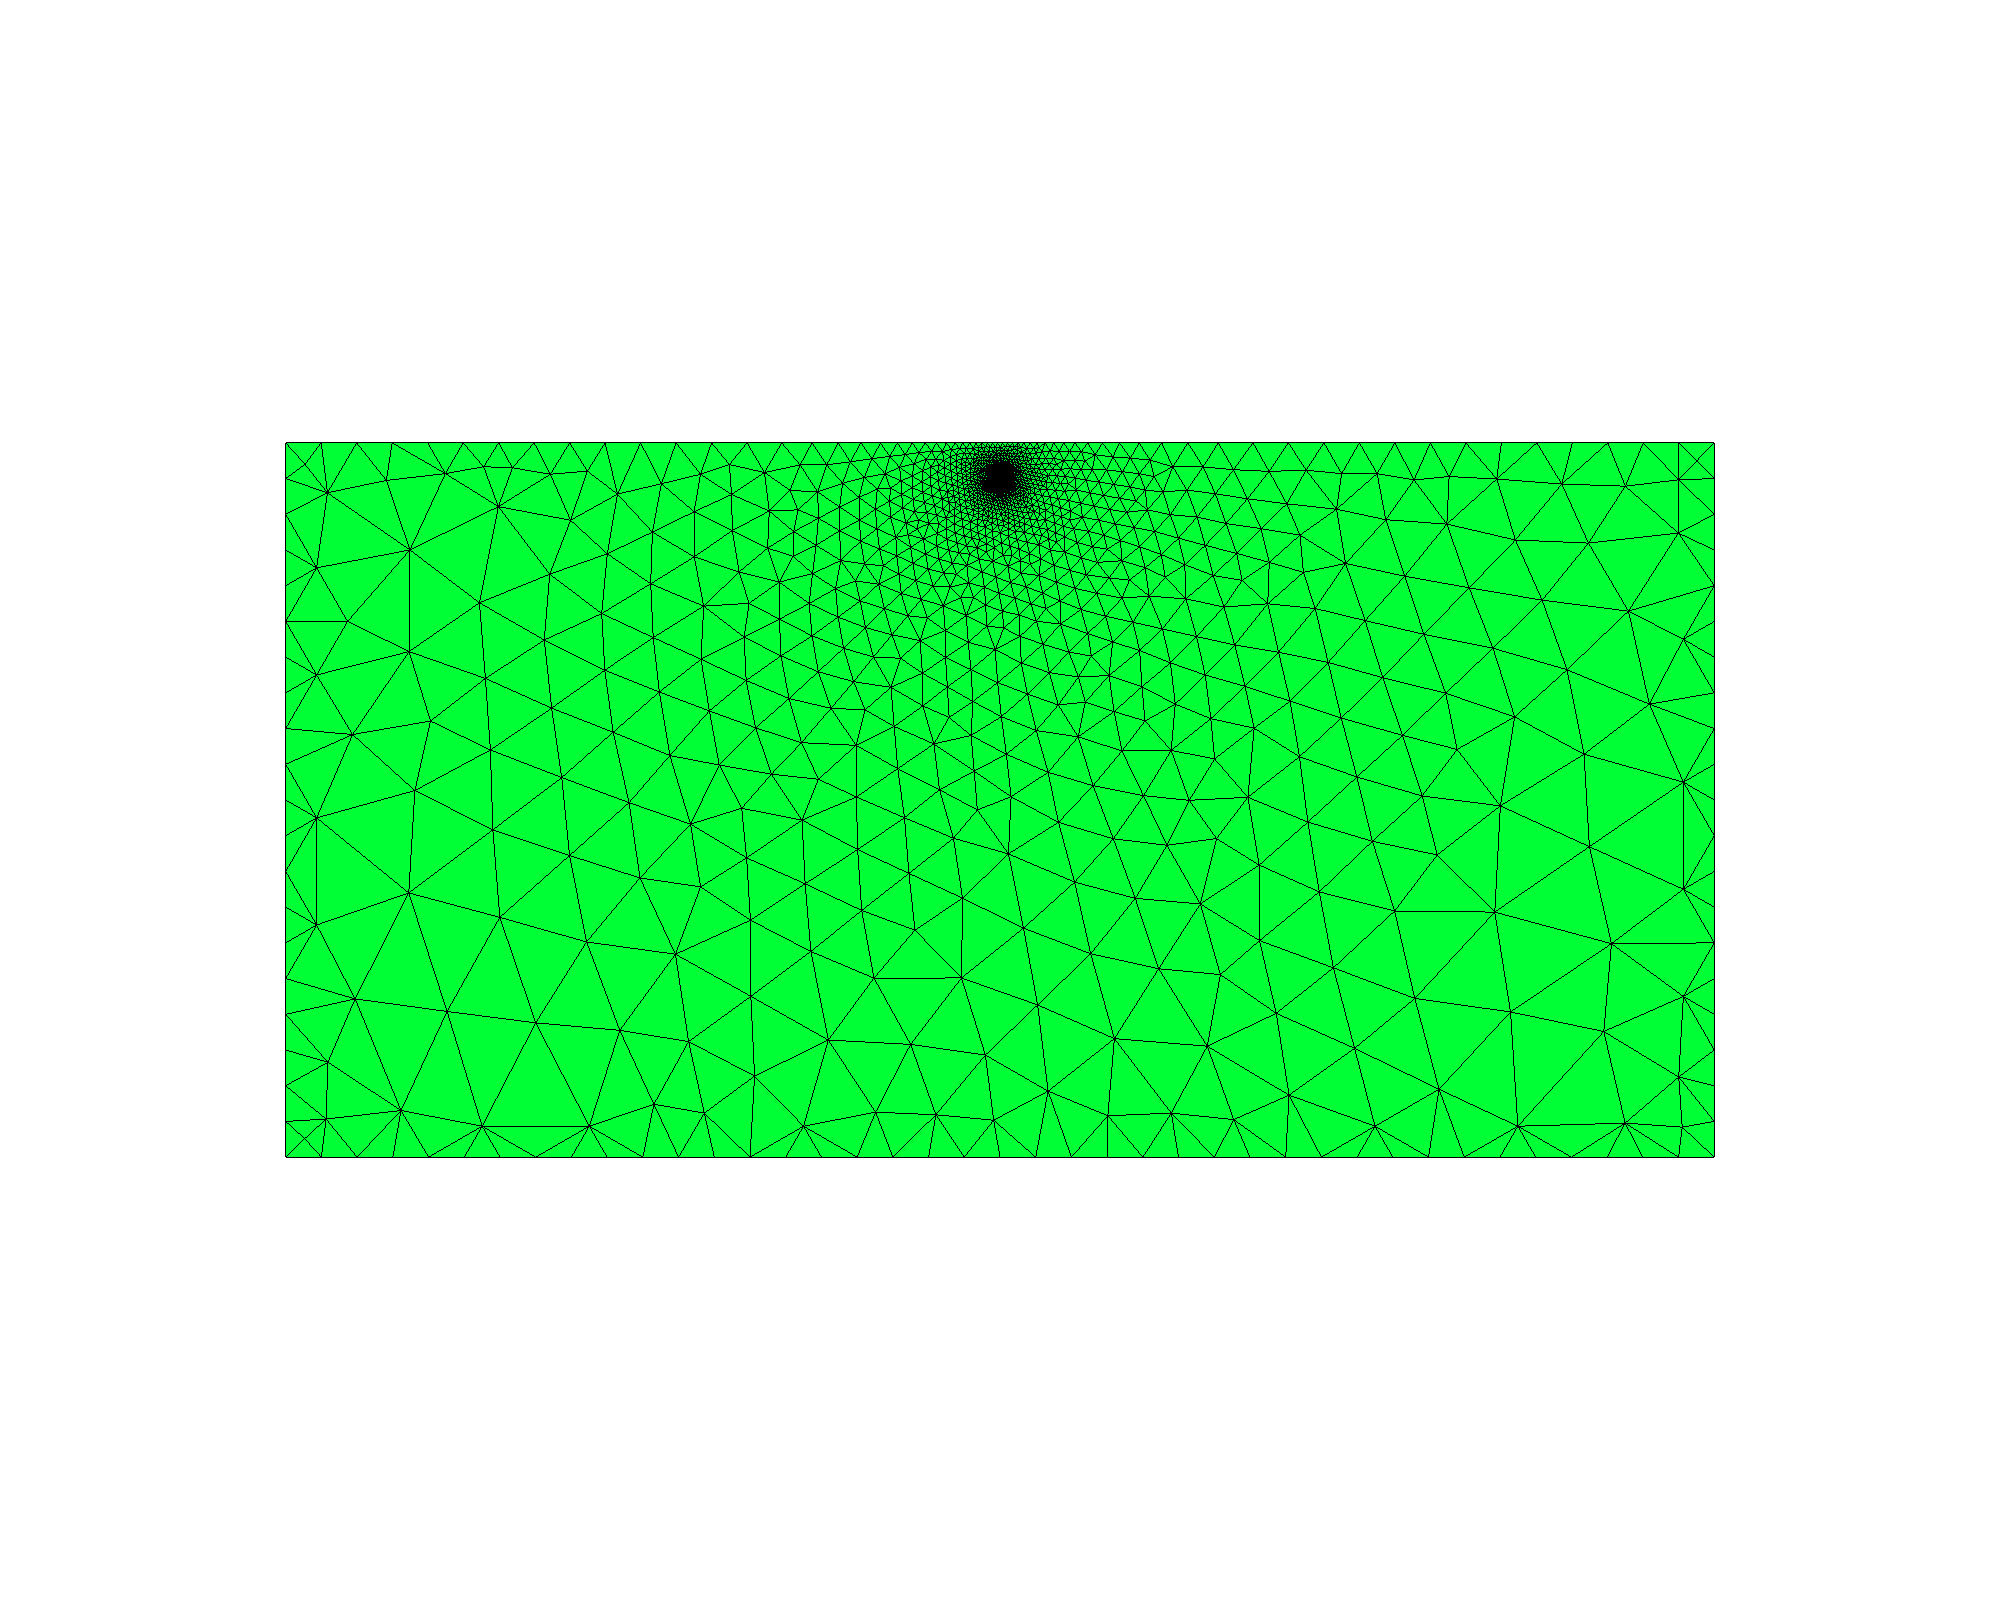
\includegraphics[width=0.75\linewidth,trim=280 438 280 438,clip]{mesh_domain.png}\end{center}

\codeguide{\setupfile{cable.geo}: thermal rectangle, groups 98, 130, 132, mesh Field 2.
\setupfile{parameters.pro}: \texttt{BurialDepth}, \texttt{hConv}, \texttt{ThermalHalfWidth},
\texttt{ThermalDepth}, \texttt{kSoil}, \texttt{kPoly}, \texttt{kAl}, \texttt{kCu}.}
{\textbf{Run} (\texttt{MagnetoThermal}).}{\texttt{res/surface\_heat\_W\_m.dat}: heat through the surface.}

\section*{Q4.3 Ambient temperature, mesh and domain size}
\assignmentquestion{\QuestionFourThree}
\answer{\AnsFourThree}
\begin{center}\small
\begin{tabular}{@{}lrrr@{}}\toprule
\(\sigma(T)\) model & \(T_{\max}\) [\(^\circ\)C] & surface \(T_{\max}\) [\(^\circ\)C] & iterations\\\midrule
MeshFactor 2 & \Tcnlcoarse & \Tsnlcoarse & \Nitnlcoarse\\
MeshFactor 1 (default) & \Tcnl & \Tsnl & \Nitnl\\
MeshFactor 0.5 & \Tcnlfine & \Tsnlfine & \Nitnlfine\\\midrule
Domain \(\pm10\) m, 10 m deep & \Tcnldomten & \Tsnldomten & \Nitnldomten\\
Domain \(\pm20\) m, 20 m deep (default) & \Tcnl & \Tsnl & \Nitnl\\
Domain \(\pm40\) m, 40 m deep & \Tcnldomforty & \Tsnldomforty & \Nitnldomforty\\\bottomrule
\end{tabular}
\end{center}
\begin{center}% Shared pgfplots style for the report and the slides. \figw / \figh set the size.
\providecommand{\figw}{0.95\linewidth}\providecommand{\figh}{5.2cm}
\providecommand{\datadir}{data}
\ifdefined\figwlen\else\newlength\figwlen\fi\setlength{\figwlen}{\figw}
\pgfplotsset{every axis/.append style={width=\figw,height=\figh,grid=major,
  grid style={gray!25},tick label style={font=\scriptsize},label style={font=\small},
  legend style={font=\scriptsize,draw=none,fill=white,fill opacity=0.85,text opacity=1}}}
\definecolor{cA}{HTML}{254C58}\definecolor{cB}{HTML}{D1495B}\definecolor{cC}{HTML}{EDAE49}
% Q4.3: hot spot versus mesh density and thermal domain size (sigma(T), 350 A).
\begin{tikzpicture}
\begin{axis}[name=m,width=0.44\linewidth,height=4.6cm,xmode=log,x dir=reverse,xlabel={MeshFactor (smaller = finer)},
  ylabel={$T_{\max}$ [$^\circ$C]},xtick={0.5,1,2},xticklabels={0.5,1,2},ymin=90.5,ymax=94,xmin=0.4,xmax=2.5,
  grid=major,grid style={gray!25},tick label style={font=\scriptsize}]
\addplot[cA,thick,mark=*] coordinates {(2,\Tcnlcoarse) (1,\Tcnl) (0.5,\Tcnlfine)};
\end{axis}
\begin{axis}[at={(m.east)},anchor=west,xshift=14mm,width=0.44\linewidth,height=4.6cm,xmode=log,
  xlabel={Thermal domain half-width = depth [m]},xtick={10,20,40},xticklabels={10,20,40},ymin=90.5,ymax=94,
  xmin=8,xmax=50,grid=major,grid style={gray!25},tick label style={font=\scriptsize}]
\addplot[cB,thick,mark=square*] coordinates {(10,\Tcnldomten) (20,\Tcnl) (40,\Tcnldomforty)};
\end{axis}
\end{tikzpicture}

\figcap{Hot spot versus mesh density (left) and thermal domain size (right).}\end{center}
The fine-mesh change is under 1\,\% of the temperature rise. The remaining error comes mostly from
the soil, where linear elements grow to metres, and from the screen losses (Section 3). The number of
coupling iterations does not change. A domain that is too small is \emph{non-conservative}.

\codeguide{\setupfile{parameters.pro}: \texttt{MeshFactor}, \texttt{ThermalHalfWidth}, \texttt{ThermalDepth}.}
{Gmsh: open \tfile, \textbf{Mesh > Mesh factor} = 2, 0.5; \textbf{Thermal > Thermal domain half-width} and \textbf{depth} = 10, 40; \textbf{Run}.
\runall: cases \texttt{nl-coarse}, \texttt{nl-fine}, \texttt{nl-dom10}, \texttt{nl-dom40}.}{\texttt{Tmax\_conductor.dat}.}

\section*{Q4.4 Temperature in the cable and hot spot}
\assignmentquestion{\QuestionFourFour}
\answer{\AnsFourFour}
\begin{center}
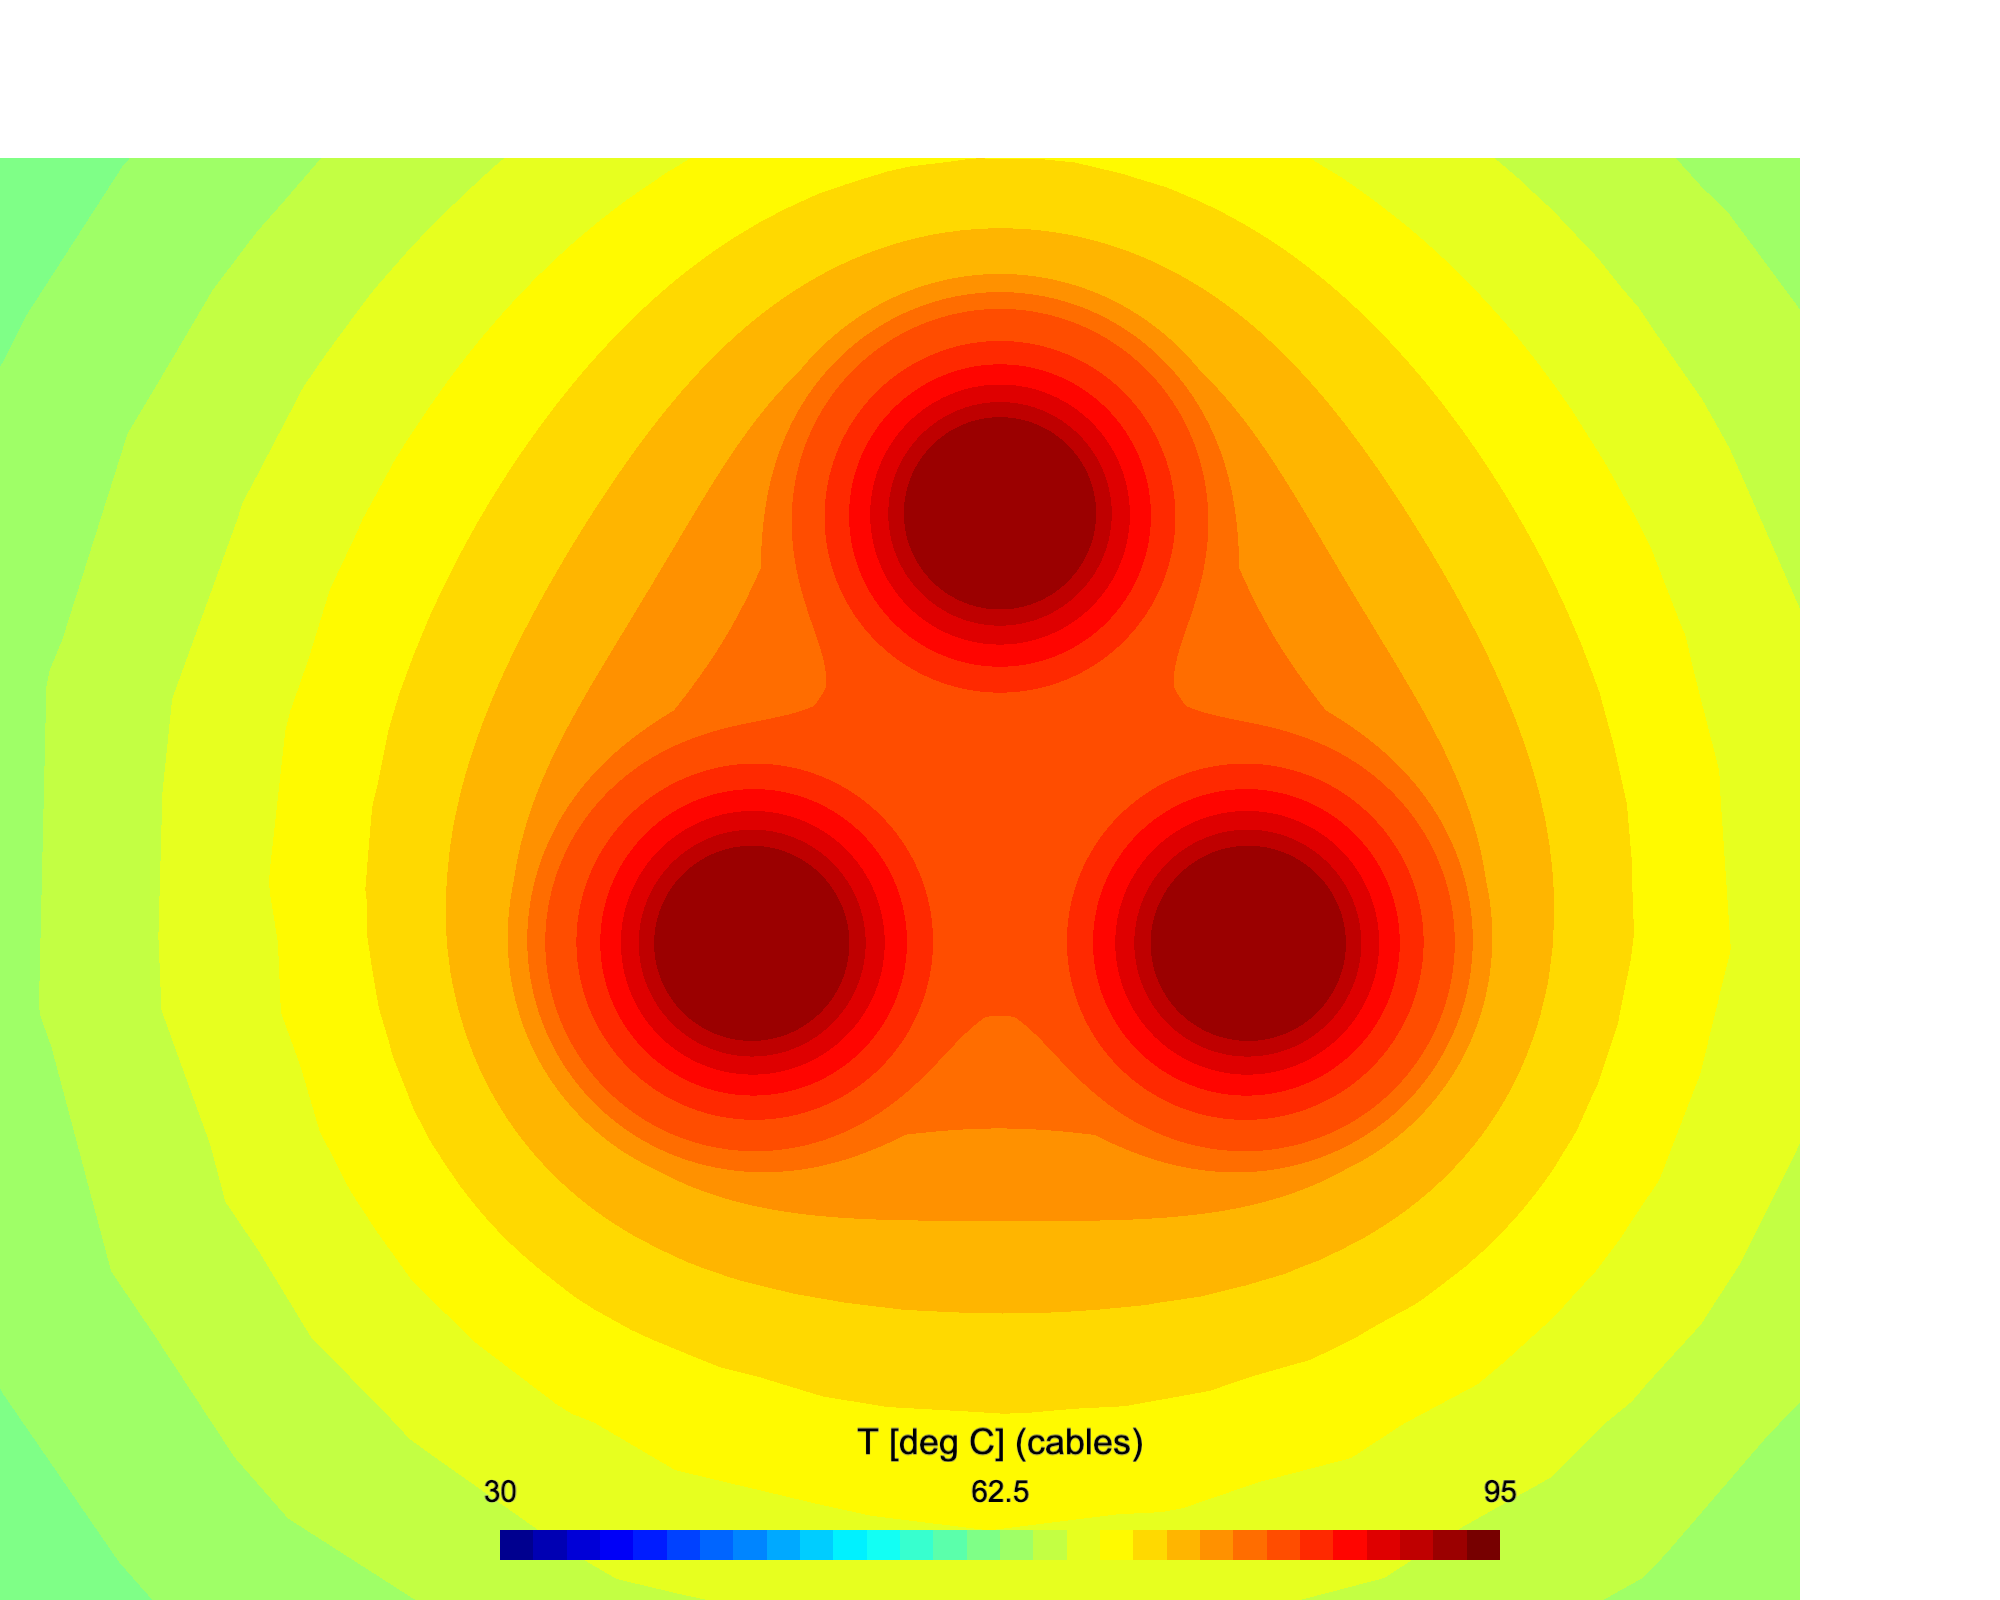
\includegraphics[width=0.47\linewidth,trim=150 0 150 0,clip]{t_cables_nl.png}\hfill
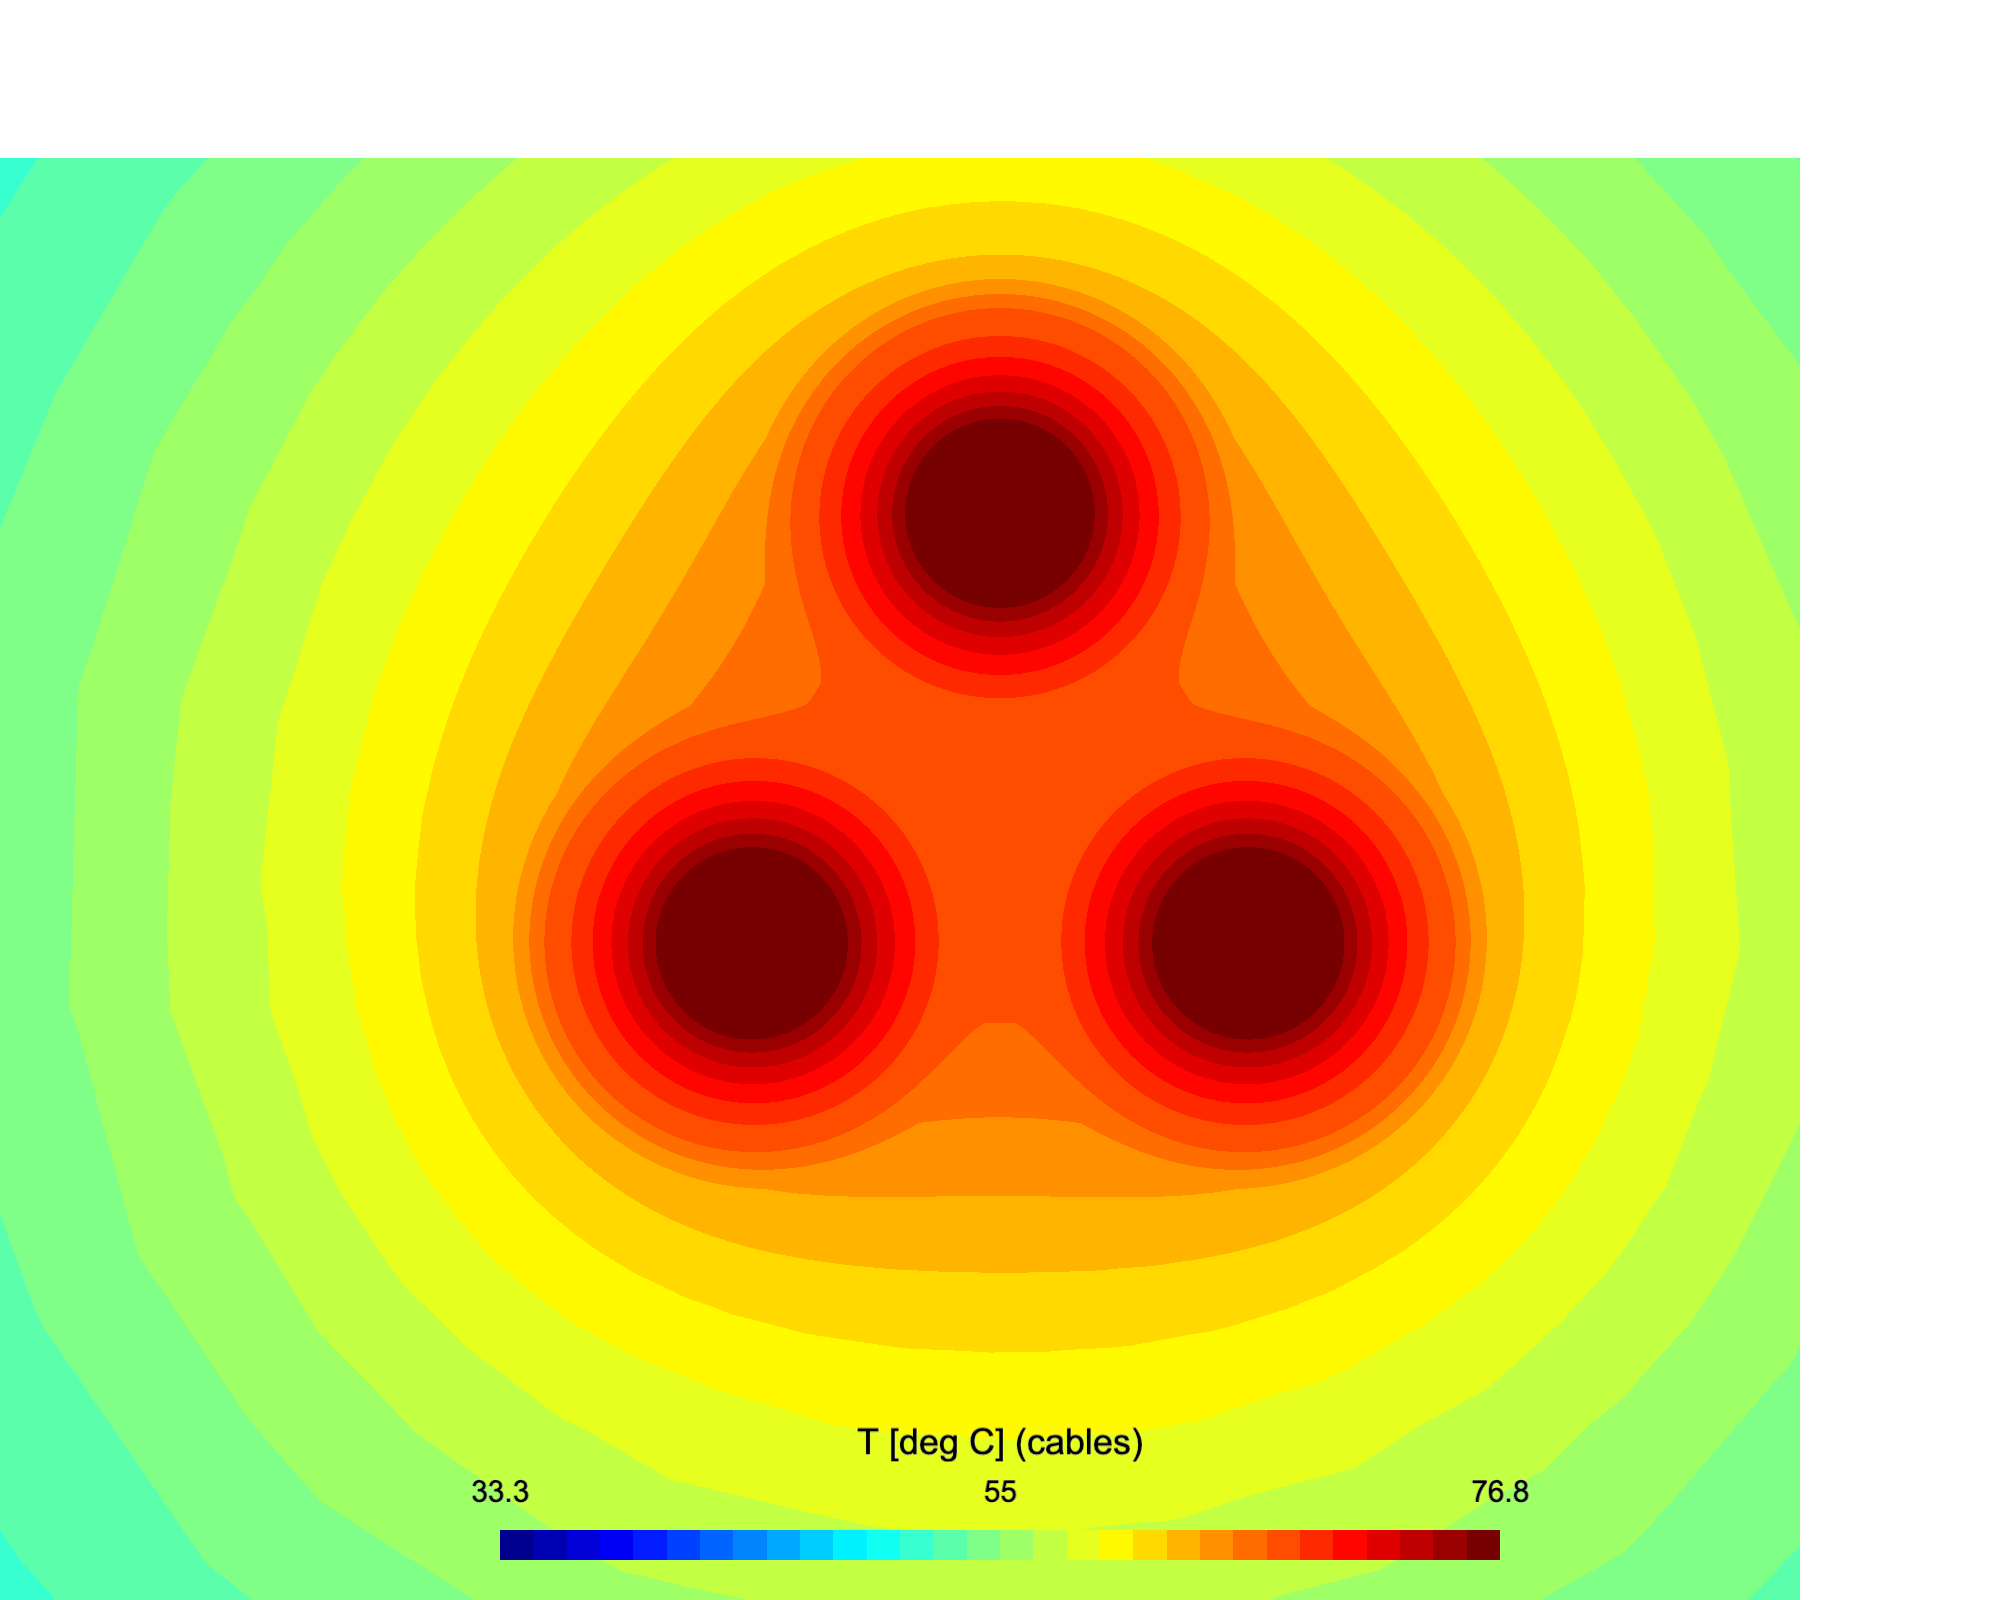
\includegraphics[width=0.47\linewidth,trim=150 0 150 0,clip]{t_cables_lin.png}\\
{\small \(\sigma(T)\) (left) and linear (right) temperature in the cable area, same colour scale (30--95\,\(^\circ\)C)}
\end{center}
B and C both reach \TcB\,\(^\circ\)C; the three phase losses are equal to \PhaseSym\,\%, so the mutual
heating is symmetric. The aluminium is isothermal thanks to \(\kappa=237\) W/(m\,K); the drop across
the XLPE corresponds to the IEC resistance \(T_1\). The 90\,\(^\circ\)C limit for XLPE is NKT's and IEC's. The uncertainties: \(h\) (Q4.5: \(\pm1\) K),
the filler conductivity (halving it adds \dTfiller\ K) and the soil. The linear model gives
\Tclin\,\(^\circ\)C (Q4.8).

\codeguide{\tfile: \texttt{The\_Values} (registers 4, 6--8).}{\textbf{Run}.}
{\texttt{res/Tmax\_conductor.dat}, \texttt{res/T\_cables.pos}.}

\section*{Q4.5 Temperature around the cable and at the ground surface}
\assignmentquestion{\QuestionFourFive}
\answer{\AnsFourFive}
\begin{center}
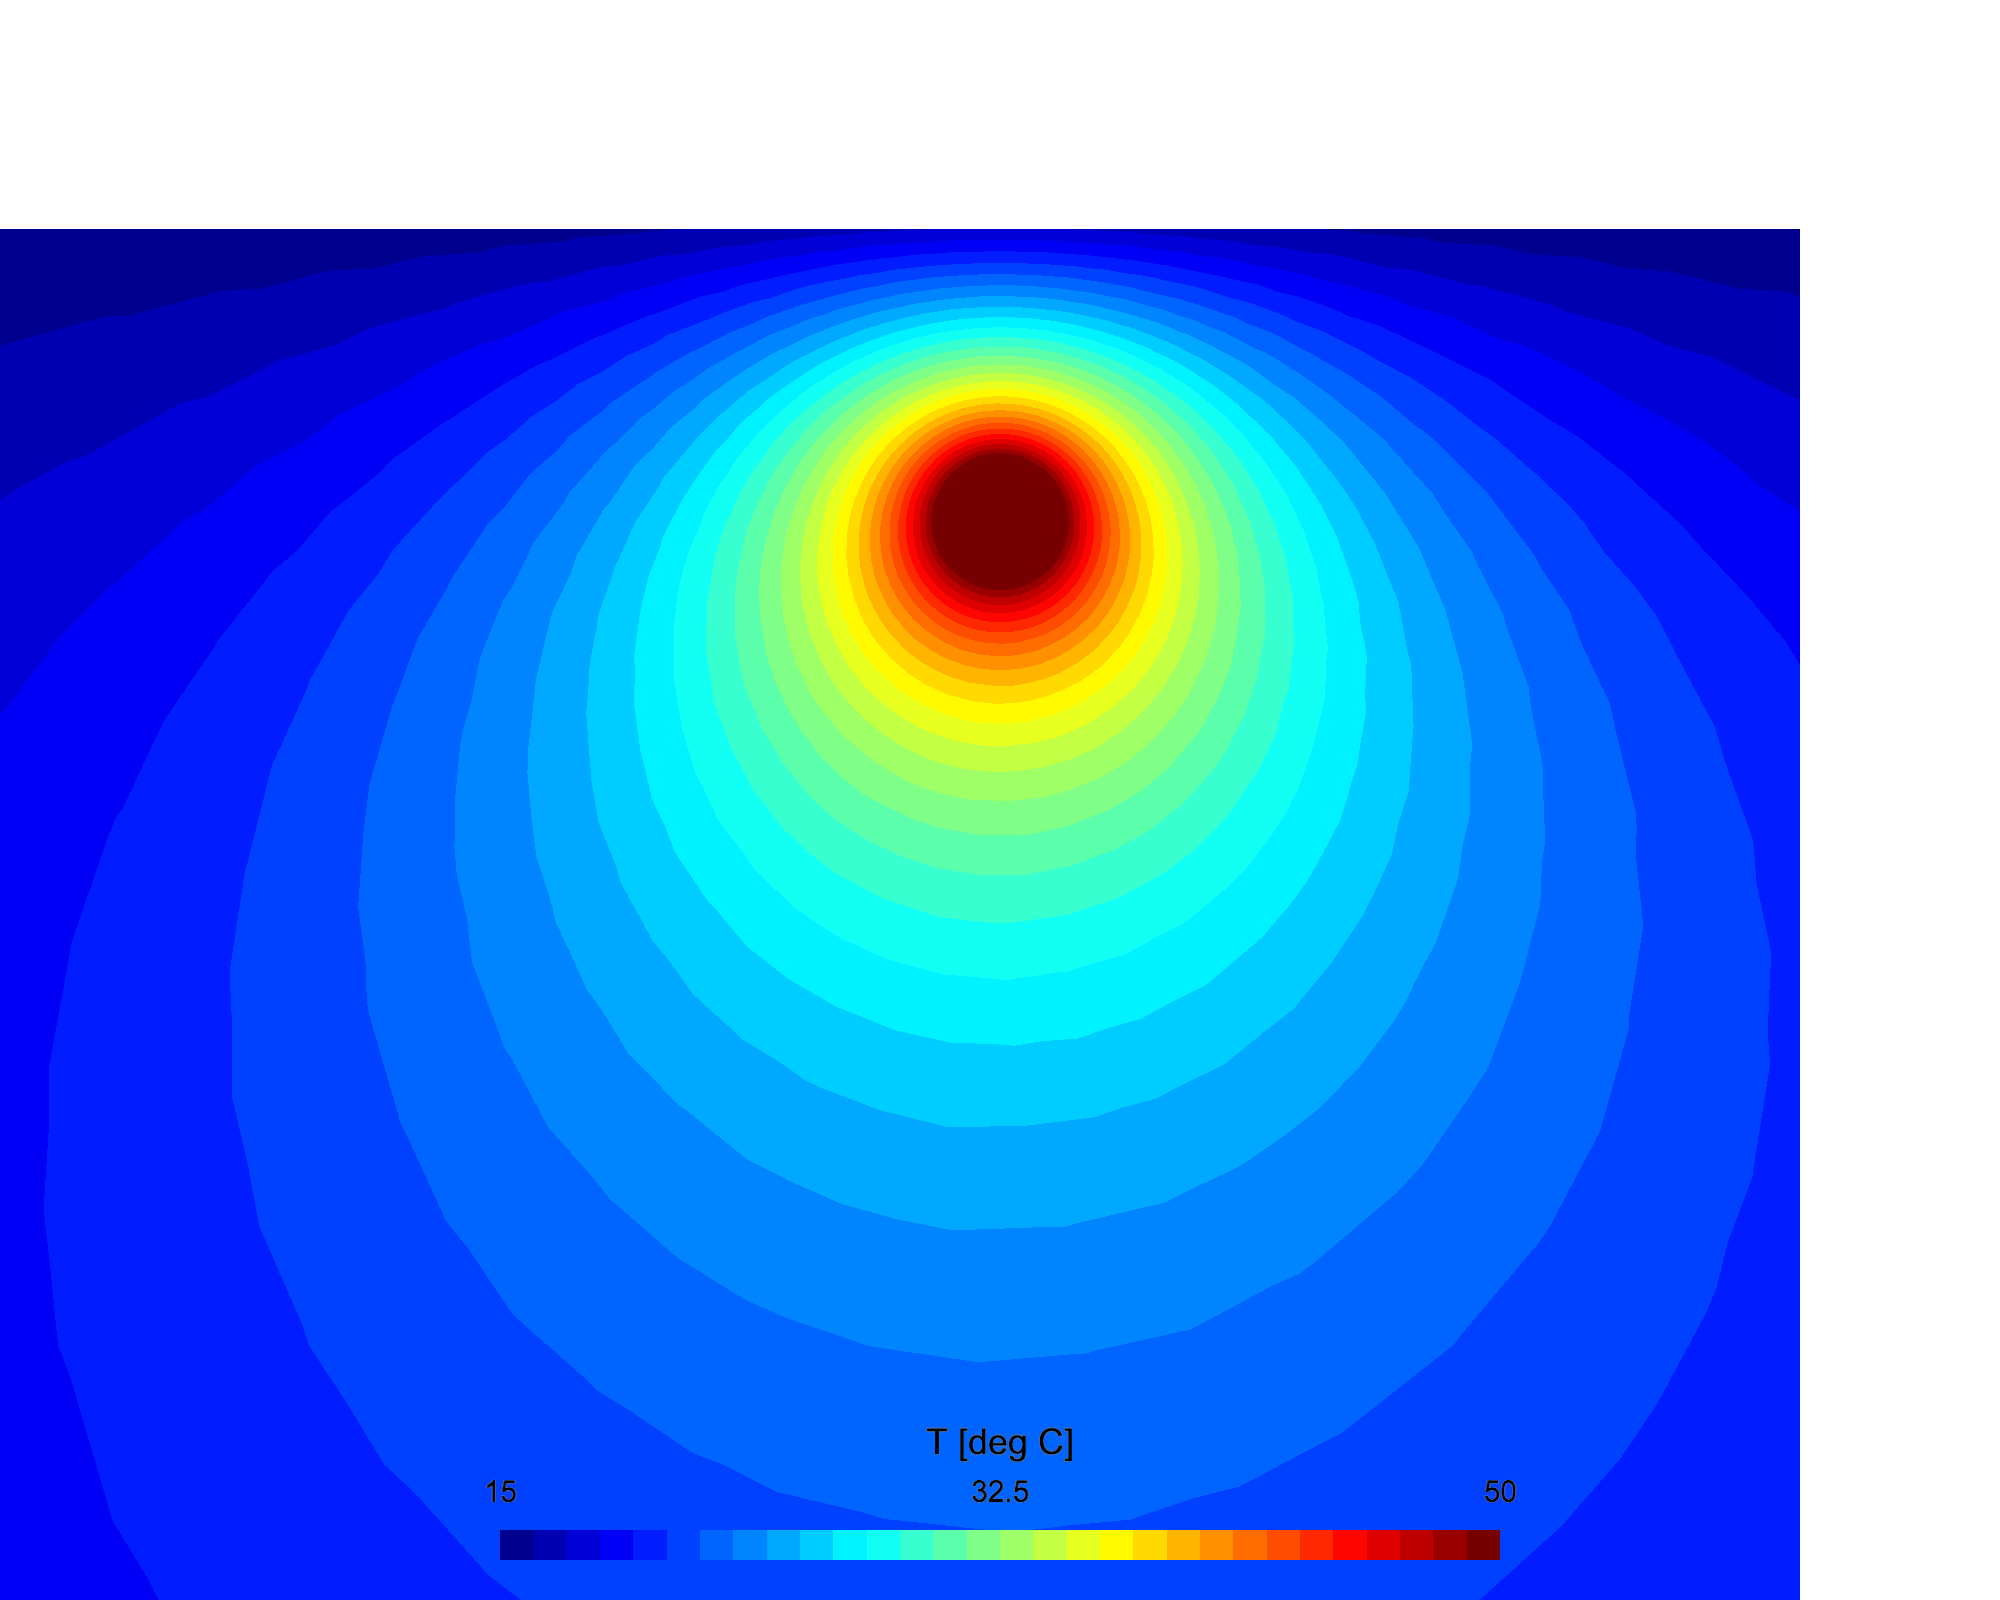
\includegraphics[width=0.38\linewidth,trim=150 0 150 0,clip]{t_soil_nl.png}\hfill
\begin{minipage}[b]{0.58\linewidth}\def\figw{\linewidth}\def\figh{5cm}
% Shared pgfplots style for the report and the slides. \figw / \figh set the size.
\providecommand{\figw}{0.95\linewidth}\providecommand{\figh}{5.2cm}
\providecommand{\datadir}{data}
\ifdefined\figwlen\else\newlength\figwlen\fi\setlength{\figwlen}{\figw}
\pgfplotsset{every axis/.append style={width=\figw,height=\figh,grid=major,
  grid style={gray!25},tick label style={font=\scriptsize},label style={font=\small},
  legend style={font=\scriptsize,draw=none,fill=white,fill opacity=0.85,text opacity=1}}}
\definecolor{cA}{HTML}{254C58}\definecolor{cB}{HTML}{D1495B}\definecolor{cC}{HTML}{EDAE49}
% Q4.5: temperature along the ground surface (sigma(T) model, 350 A).
\begin{tikzpicture}\begin{axis}[xlabel={$x$ along the ground surface [m]},
  ylabel={$T$ [$^\circ$C]},xmin=-6,xmax=6,ymin=14.8,legend cell align=left,legend style={at={(0.5,1.03)},anchor=south,legend columns=2,/tikz/every even column/.append style={column sep=6pt}}]
\addplot[cB,thick] table[x=x,y=T,col sep=comma]{\datadir/surface_h5.csv};
\addplot[cA,thick] table[x=x,y=T,col sep=comma]{\datadir/surface_nl.csv};
\addplot[cC,thick] table[x=x,y=T,col sep=comma]{\datadir/surface_h20.csv};
\addplot[black,dashed,domain=-6:6] {15};
\legend{$h=5$,$h=10$ (baseline),$h=20$ W/(m$^2$K),isothermal $T_{\rm amb}$}
\end{axis}\end{tikzpicture}
\end{minipage}
\end{center}
\begin{center}\small
\begin{tabular}{@{}lrr@{}}\toprule
Ground surface condition & surface \(T_{\max}\) [\(^\circ\)C] & conductor \(T_{\max}\) [\(^\circ\)C]\\\midrule
Convection \(h=5\) W/(m\(^2\)K) & \Tsnlhfive & \Tcnlhfive\\
Convection \(h=10\) (baseline) & \Tsnl & \Tcnl\\
Convection \(h=20\) & \Tsnlhtwenty & \Tcnlhtwenty\\
Dirichlet \(T=T_{\rm amb}\) & 15.00 & \Tcnliso\\\bottomrule
\end{tabular}
\end{center}
The isothermal surface is only slightly non-conservative because \(1/h=0.1\) m\(^2\)K/W is small
compared with the soil resistance between cable and surface.

\codeguide{\tfile: \texttt{Flag\_SurfaceBC}, \texttt{hConv}.}
{Gmsh: \textbf{Thermal > Ground surface condition} = Isothermal, or \textbf{Thermal > Surface heat transfer coefficient} = 5, 20; \textbf{Run}.
\runall: cases \texttt{nl-iso}, \texttt{nl-h5}, \texttt{nl-h20}.}
{\texttt{res/Tmax\_surface.dat}, \texttt{res/T\_surface\_profile.txt} (x, y, z, T).}

\section*{Q4.6 Validation against IEC 60287 and the datasheet}
\assignmentquestion{\QuestionFourSix}
\answer{\AnsFourSix}
IEC 60287 thermal ladder for one cable of the trefoil (no armour, no dielectric loss):
\[
 \theta_c-\theta_{\rm amb}=W_c\big[T_1+(1+\lambda_1)(T_3+T_4)\big],\qquad W_c=I^2R_{AC}(\theta_c).
\]
\begin{center}\small
\begin{tabular}{@{}lll@{}}\toprule
Quantity & Formula & Value\\\midrule
\(T_1\) insulation incl.\ semicons + inner filler [UNCC] & \(\frac{\rho}{2\pi}\ln(17.4/7.4)\), \(\rho=3.5\) & \IecTone\ K\,m/W\\
\(T_3\) outer filler + sheath [KTH] & \(\frac{\rho}{2\pi}\ln(21.5/17.85)\) & \IecTthree\ K\,m/W\\
\(T_4\) soil, touching trefoil [Karlstrand] & \(\frac{1.5}{\pi}\rho_T[\ln(2u)-0.630]\), \(u=2L/D_e=\IecU\) & \IecTfour\ K\,m/W\\
\(R_{AC}(\theta_c)\) & \(R_{20}(1+\alpha(\theta_c-20))(1+y_s+y_p)\) & \IecRcondHot\ \(\Omega\)/km\\
\(\lambda_1\) (screen at \IecThetaS\,\(^\circ\)C) & \(\frac{R_s/R}{1+(R_s/X)^2}\) & \IecLamHot\,\%\\\bottomrule
\end{tabular}
\end{center}
\begin{center}% Q4.6: IEC 60287 thermal ladder for one cable (heat flows from left to right).
\begin{tikzpicture}[font=\small,>=Stealth,res/.style={draw,thick,fill=white,minimum width=12mm,minimum height=4mm}]
\coordinate (c) at (0,0); \coordinate (s) at (3.2,0); \coordinate (e) at (6.4,0); \coordinate (a) at (9.6,0);
\draw[thick] (c) -- (a);
\node[res] at (1.6,0) {\(T_1\)}; \node[res] at (4.8,0) {\(T_3\)}; \node[res] at (8.0,0) {\(T_4\)};
\foreach \p/\l/\w in {c/{\(\theta_c\)}/left, s/{\(\theta_s\)}/{above right}, e/{\(\theta_e\)}/above, a/{\(\theta_{\rm amb}=15\,^\circ\)C}/right}
  {\fill (\p) circle (1.5pt); \node[\w=2pt] at (\p) {\l};}
\draw[->,thick,cB] (0,1.0) node[above] {\(W_c=I^2R_{AC}(\theta_c)\)} -- (c);
\draw[->,thick,cC!80!black] (3.2,1.0) node[above] {\(\lambda_1W_c\) (screen)} -- (s);
\node[below=3pt,font=\footnotesize,align=center] at (1.6,-0.15) {XLPE + semicons\\ + inner filler};
\node[below=3pt,font=\footnotesize,align=center] at (4.8,-0.15) {outer filler\\ + PE};
\node[below=3pt,font=\footnotesize,align=center] at (8.0,-0.15) {soil, trefoil\\ (Kennelly)};
\end{tikzpicture}

\figcap{IEC 60287 thermal circuit of one cable: the conductor and screen losses flow through
the insulation, sheath and soil resistances to the ambient.}\end{center}
Both \(\theta_c\) at 350 A and the current for 90\,\(^\circ\)C follow by iteration.
\begin{center}\small
\begin{tabular}{@{}lrr@{}}\toprule
350 A, \(\sigma(T)\) & \(\theta_c\) [\(^\circ\)C] & ampacity at 90\,\(^\circ\)C [A]\\\midrule
NKT datasheet & 90 & 350\\
IEC 60287 (isothermal surface) & \IecTheta & \IecAmp\\
FE, isothermal surface & \Tcnliso & --\\
FE, convection \(h=10\) & \Tcnl & \Amptrefoil\\\bottomrule
\end{tabular}
\end{center}
\begin{center}\def\figw{0.75\linewidth}\def\figh{4.6cm}% Shared pgfplots style for the report and the slides. \figw / \figh set the size.
\providecommand{\figw}{0.95\linewidth}\providecommand{\figh}{5.2cm}
\providecommand{\datadir}{data}
\ifdefined\figwlen\else\newlength\figwlen\fi\setlength{\figwlen}{\figw}
\pgfplotsset{every axis/.append style={width=\figw,height=\figh,grid=major,
  grid style={gray!25},tick label style={font=\scriptsize},label style={font=\small},
  legend style={font=\scriptsize,draw=none,fill=white,fill opacity=0.85,text opacity=1}}}
\definecolor{cA}{HTML}{254C58}\definecolor{cB}{HTML}{D1495B}\definecolor{cC}{HTML}{EDAE49}
% Q4.6: conductor temperature at 350 A: datasheet, IEC 60287 and FE.
\begin{tikzpicture}\begin{axis}[xbar,bar width=11pt,xlabel={Conductor temperature at 350 A [$^\circ$C]},
  xmin=80,xmax=96,symbolic y coords={FE convection,FE isothermal,IEC 60287,NKT rating},ytick=data,
  enlarge y limits=0.18,extra x ticks={90},extra x tick labels={},
  extra x tick style={grid=major,grid style={cB,thick,dashed}},nodes near coords,nodes near coords style={font=\scriptsize}]
\addplot[fill=cA!80,draw=cA] coordinates {(\Tcnl,FE convection) (\Tcnliso,FE isothermal) (\IecTheta,IEC 60287) (90,NKT rating)};
\end{axis}\end{tikzpicture}

\figcap{Conductor temperature at the rated 350 A; dashed: the 90\,\(^\circ\)C rating temperature.}\end{center}
More on the differences: IEC uses Kennelly's image method with an empirical trefoil factor
(1.5/\(\pi\), \(-0.630\)) and treats each cable as a cylinder at a uniform surface temperature; the FE
screen losses give \(\lambda_1\approx\Psnl/\Pcnl\); and the FE domain is finite.

\codeguide{IEC values: computed and printed by \tfile\ (macro \texttt{IecAt}, the ladder loops).}
{Gmsh: \textbf{Run} (defaults), then \textbf{Thermal > Ground surface condition} = Isothermal, \textbf{Run}.
\runall: cases \texttt{nl}, \texttt{nl-iso}.}{\texttt{Tmax\_conductor.dat}, \texttt{references.txt}.}

\section*{Q4.7 Nonlinear coupling and convergence}
\assignmentquestion{\QuestionFourSeven}
\answer{\AnsFourSeven}
\textbf{Algorithm} (staggered fixed point, resolution \texttt{MagnetoThermal}): start with
\(T_0=20\,^\circ\)C everywhere; for \(k=1,2,\dots\): solve the magnetic problem with
\(\sigma(T_{k-1})\), compute \(p_k\), solve the thermal problem for \(T_k\).
The first pass (\(\sigma\) at 20\,\(^\circ\)C) is exactly the linear model.

\textbf{Criterion.} The norms come from GetDP's \texttt{GetNormIncrement} and \texttt{GetNormSolution}.
With \(T\) in \(^\circ\)C, \(10^{-6}\) corresponds to changes of order \(10^{-4}\) K at the hot spot, far below
any physical uncertainty.

\begin{center}\def\figw{0.75\linewidth}\def\figh{5.5cm}
% Shared pgfplots style for the report and the slides. \figw / \figh set the size.
\providecommand{\figw}{0.95\linewidth}\providecommand{\figh}{5.2cm}
\providecommand{\datadir}{data}
\ifdefined\figwlen\else\newlength\figwlen\fi\setlength{\figwlen}{\figw}
\pgfplotsset{every axis/.append style={width=\figw,height=\figh,grid=major,
  grid style={gray!25},tick label style={font=\scriptsize},label style={font=\small},
  legend style={font=\scriptsize,draw=none,fill=white,fill opacity=0.85,text opacity=1}}}
\definecolor{cA}{HTML}{254C58}\definecolor{cB}{HTML}{D1495B}\definecolor{cC}{HTML}{EDAE49}
% Q4.7: relative temperature increment per coupling iteration (three meshes).
\begin{tikzpicture}\begin{axis}[ymode=log,xlabel={Coupling iteration $k$},
  ylabel={$\|T_k-T_{k-1}\|_2/\|T_k\|_2$},xmin=0.5,ymax=2,legend pos=north east]
\addplot[cB,thick,mark=*,mark size=1.6pt] table[x=it,y=rel,col sep=comma]{\datadir/nl_history.csv};
\addplot[cA,mark=square,mark size=1.6pt] table[x=it,y=rel,col sep=comma]{\datadir/nl_history_coarse.csv};
\addplot[cC,thick,mark=triangle,mark size=1.8pt] table[x=it,y=rel,col sep=comma]{\datadir/nl_history_fine.csv};
\addplot[black,dashed,domain=0.5:16] {1e-6};
\legend{MeshFactor 1,MeshFactor 2,MeshFactor 0.5,tolerance $10^{-6}$}
\end{axis}\end{tikzpicture}
\end{center}
The convergence is linear: the increment drops by a constant factor \(\approx\)\,\ConvRate\ per
iteration. That factor is the sensitivity of the hot spot to itself:
\(\partial T/\partial T_{\rm prev}\approx\alpha\,\Delta T\,/(1+\alpha(T-20))\approx0.0039\times75/1.3\approx0.22\).
It would approach 1 (divergence: thermal runaway) only for a much larger temperature rise.

\codeguide{\tfile: macro \texttt{CoupledSolve} (\texttt{While}, \texttt{GetNormIncrement}),
\texttt{Flag\_NL}, \texttt{NL\_tol}, constraint \texttt{Temperature} (\texttt{Type Init}).}
{\textbf{Run}; the log prints every iteration.}{\texttt{res/convergence.txt} (iteration, increment).}

\section*{Q4.8 Linear versus \texorpdfstring{\(\sigma(T)\)}{sigma(T)}}
\assignmentquestion{\QuestionFourEight}
\answer{\AnsFourEight}
\begin{center}\small
\begin{tabular}{@{}lrrr@{}}\toprule
Quantity & linear (20\,\(^\circ\)C) & \(\sigma(T)\) & change\\\midrule
Conductor losses [kW/km] & \Pclin & \Pcnl & \dPcNL\,\%\\
Screen losses [kW/km] & \Pslin & \Psnl & \dPsNL\,\%\\
Total losses [kW/km] & \Ptlin & \Ptnl & \dPtNL\,\%\\
\(R_{AC}\) [\(\Omega\)/km] & \Raclin & \Racnl & \dRacNL\,\%\\
\(L\) [mH/km] & \Llin & \Lnl & \dLNL\,\%\\
Screen current [A] & \Islin & \Isnl & \\
Hot spot [\(^\circ\)C] & \Tclin & \Tcnl & \dTcNL\ K\\
Max.\ surface temperature [\(^\circ\)C] & \Tslin & \Tsnl & \\\bottomrule
\end{tabular}
\end{center}
\begin{center}\def\figw{0.75\linewidth}\def\figh{4.8cm}% Shared pgfplots style for the report and the slides. \figw / \figh set the size.
\providecommand{\figw}{0.95\linewidth}\providecommand{\figh}{5.2cm}
\providecommand{\datadir}{data}
\ifdefined\figwlen\else\newlength\figwlen\fi\setlength{\figwlen}{\figw}
\pgfplotsset{every axis/.append style={width=\figw,height=\figh,grid=major,
  grid style={gray!25},tick label style={font=\scriptsize},label style={font=\small},
  legend style={font=\scriptsize,draw=none,fill=white,fill opacity=0.85,text opacity=1}}}
\definecolor{cA}{HTML}{254C58}\definecolor{cB}{HTML}{D1495B}\definecolor{cC}{HTML}{EDAE49}
% Q4.8: change from the linear (sigma at 20 C) to the sigma(T) model, % (350 A).
\begin{tikzpicture}\begin{axis}[xbar,bar width=10pt,xlabel={Change linear \(\rightarrow\) \(\sigma(T)\) [\%]},xmin=-38,xmax=48,
  symbolic y coords={L,Rac,Pt,Ps,Pc},ytick={L,Rac,Pt,Ps,Pc},yticklabels={$L$,$R_{AC}$,total loss,screen loss,conductor loss},
  enlarge y limits=0.15,nodes near coords,nodes near coords style={font=\scriptsize},
  extra x ticks={0},extra x tick labels={},extra x tick style={grid=major,grid style={black}}]
\addplot[fill=cA!80,draw=cA] table[y=q,x=change,col sep=comma]{\datadir/nl_change.csv};
\end{axis}\end{tikzpicture}

\figcap{Relative change from the linear to the \(\sigma(T)\) model: losses and \(R_{AC}\) rise by a quarter,
the screen loss falls, \(L\) barely moves; the hot spot rises by \dTcNL\ K.}\end{center}
With imposed current the conductor loss grows almost in proportion to the resistivity, and so do
\(R_{AC}\) and every temperature rise. The screen loss falls because, with \(R_s\gg X\),
\(\lambda_1\approx X^2/(R_sR)\). \(\mathbf B\) and \(L\) change only through the small screen reaction and the
current distribution, which becomes slightly more uniform as \(\delta\propto1/\sqrt\sigma\) grows.
\begin{center}
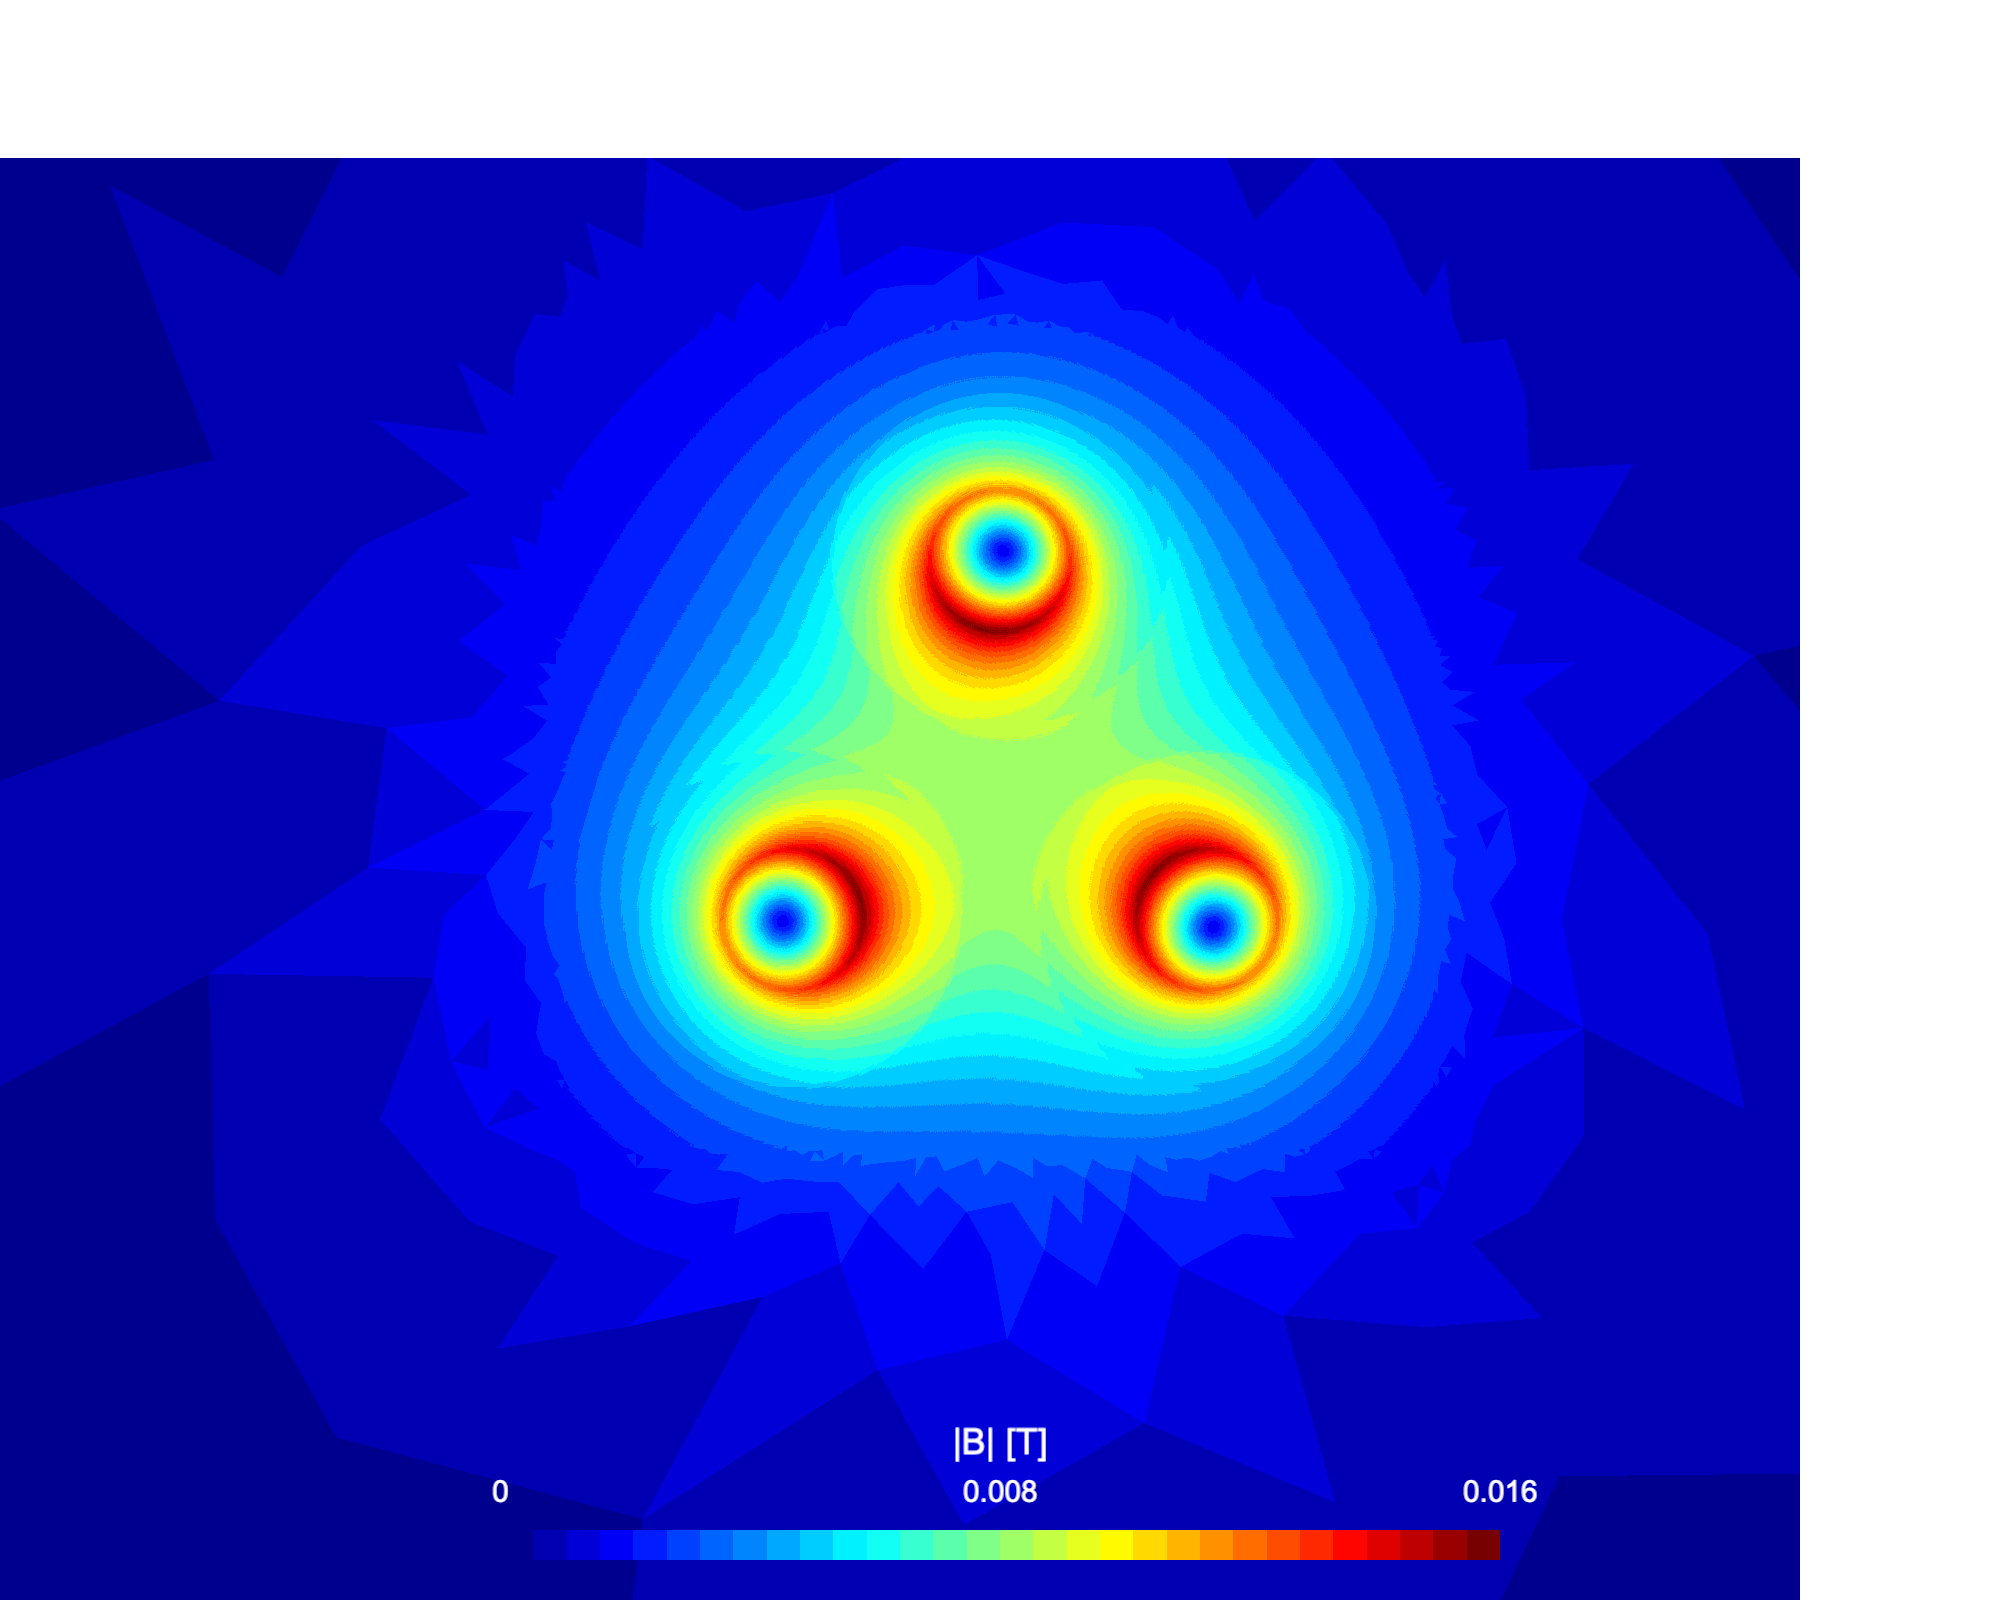
\includegraphics[width=0.23\linewidth,trim=150 0 150 0,clip]{m_b.png}\hfill
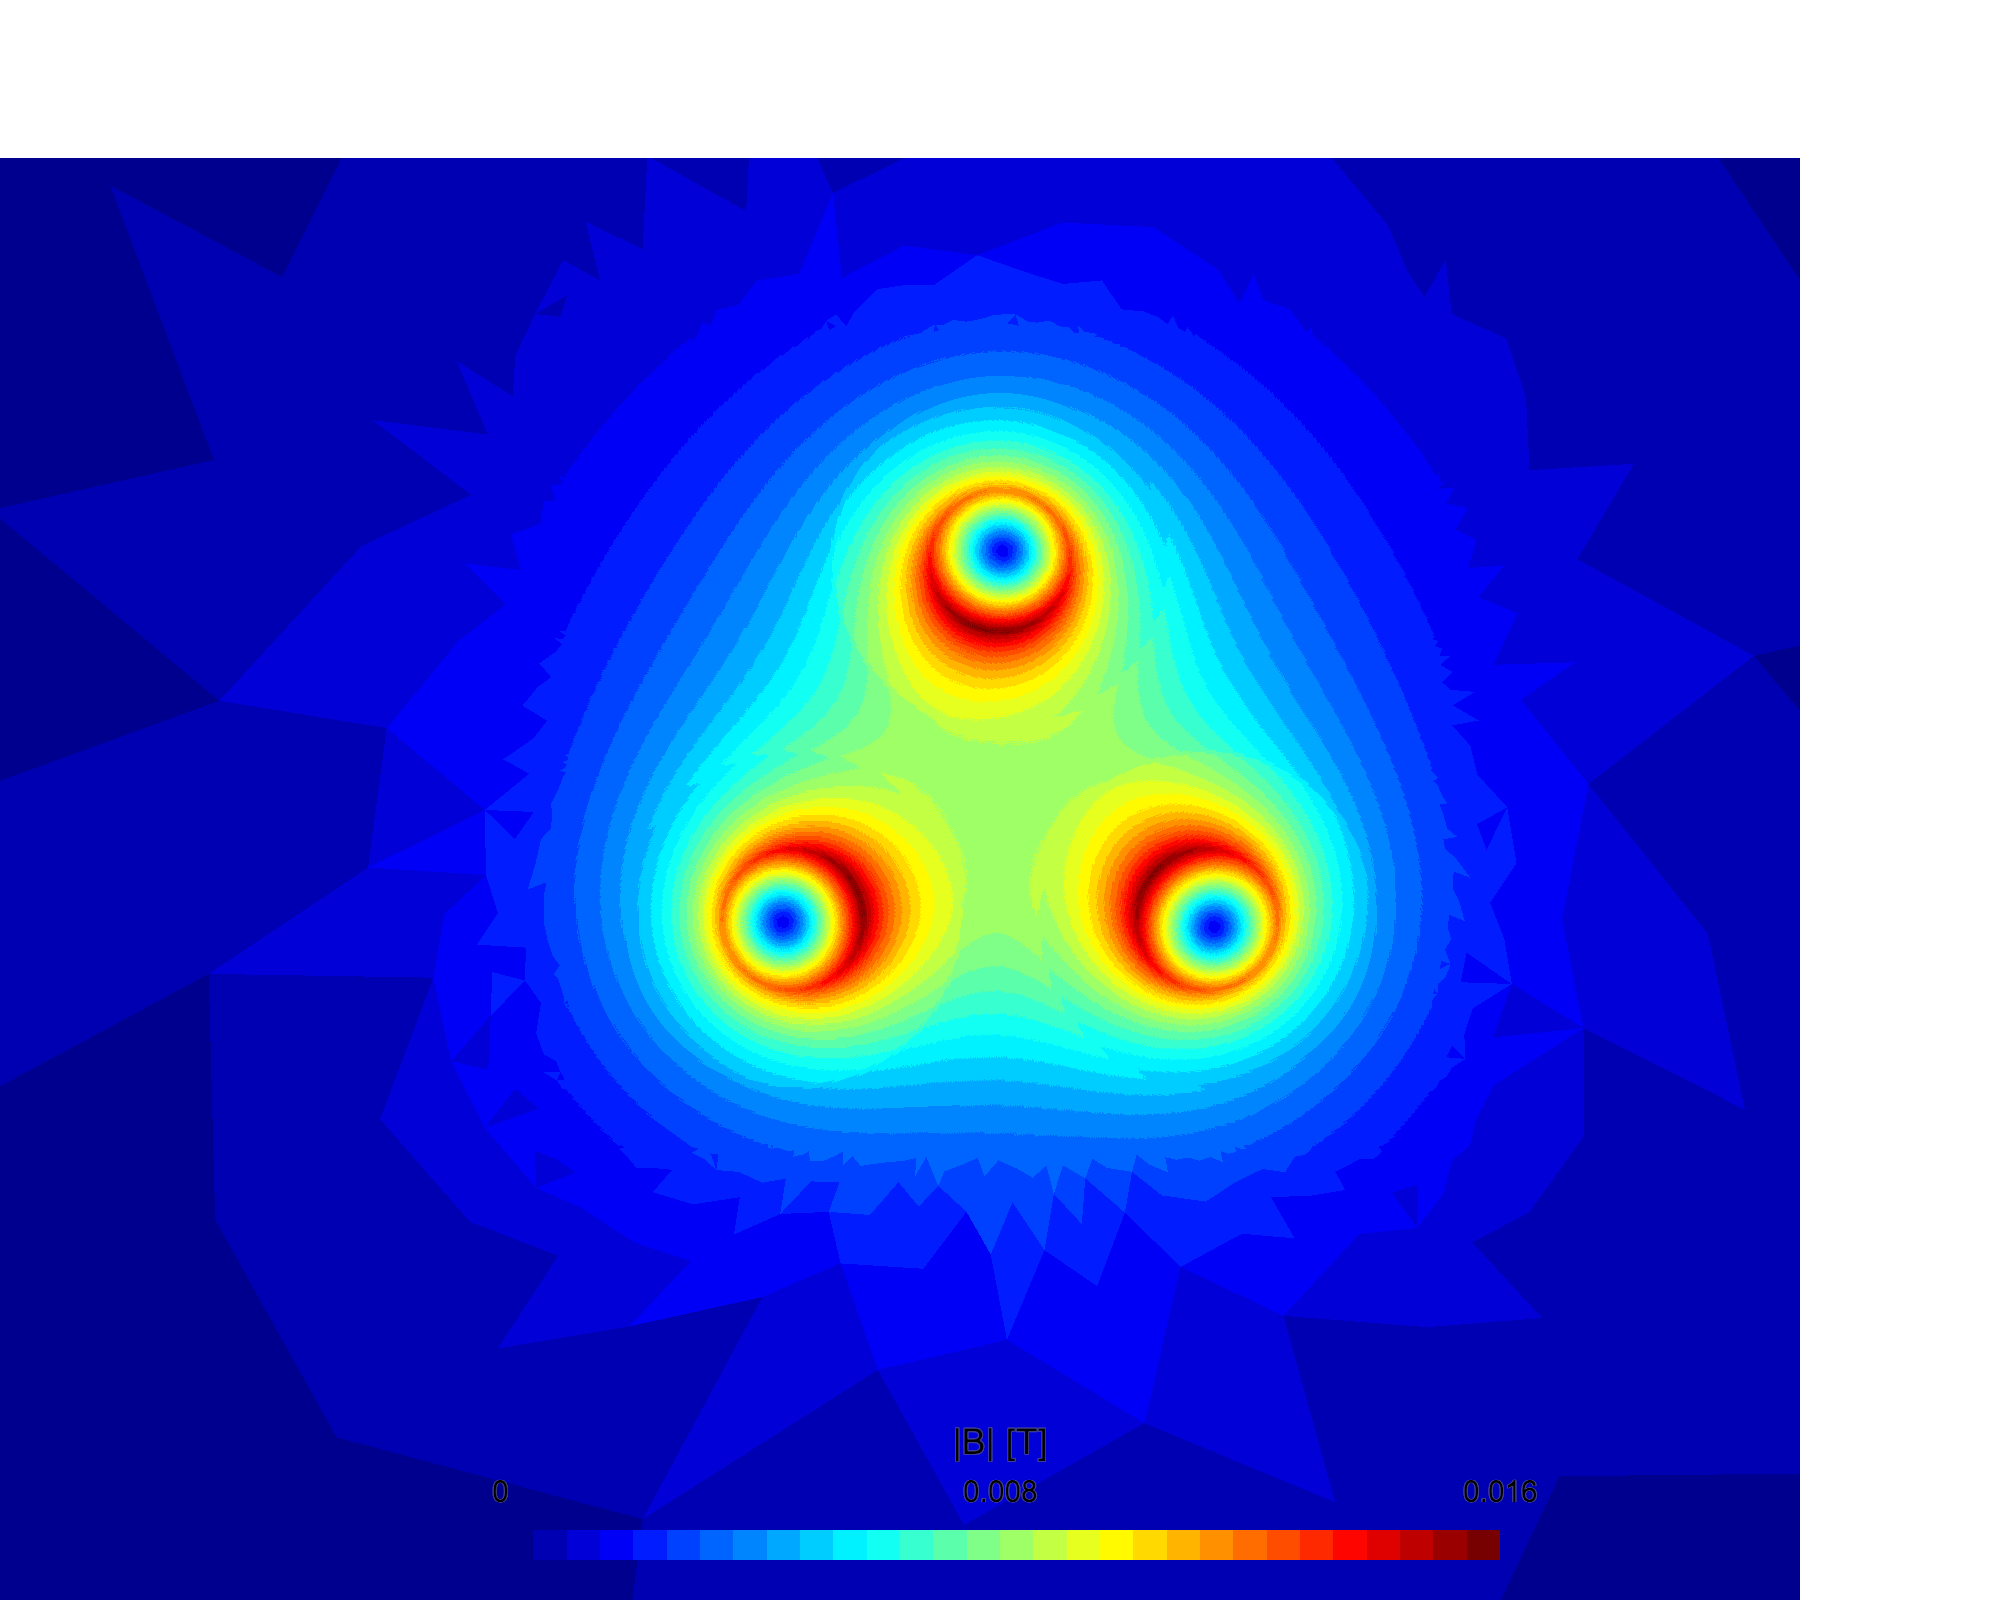
\includegraphics[width=0.23\linewidth,trim=150 0 150 0,clip]{m_b_nl.png}\hfill
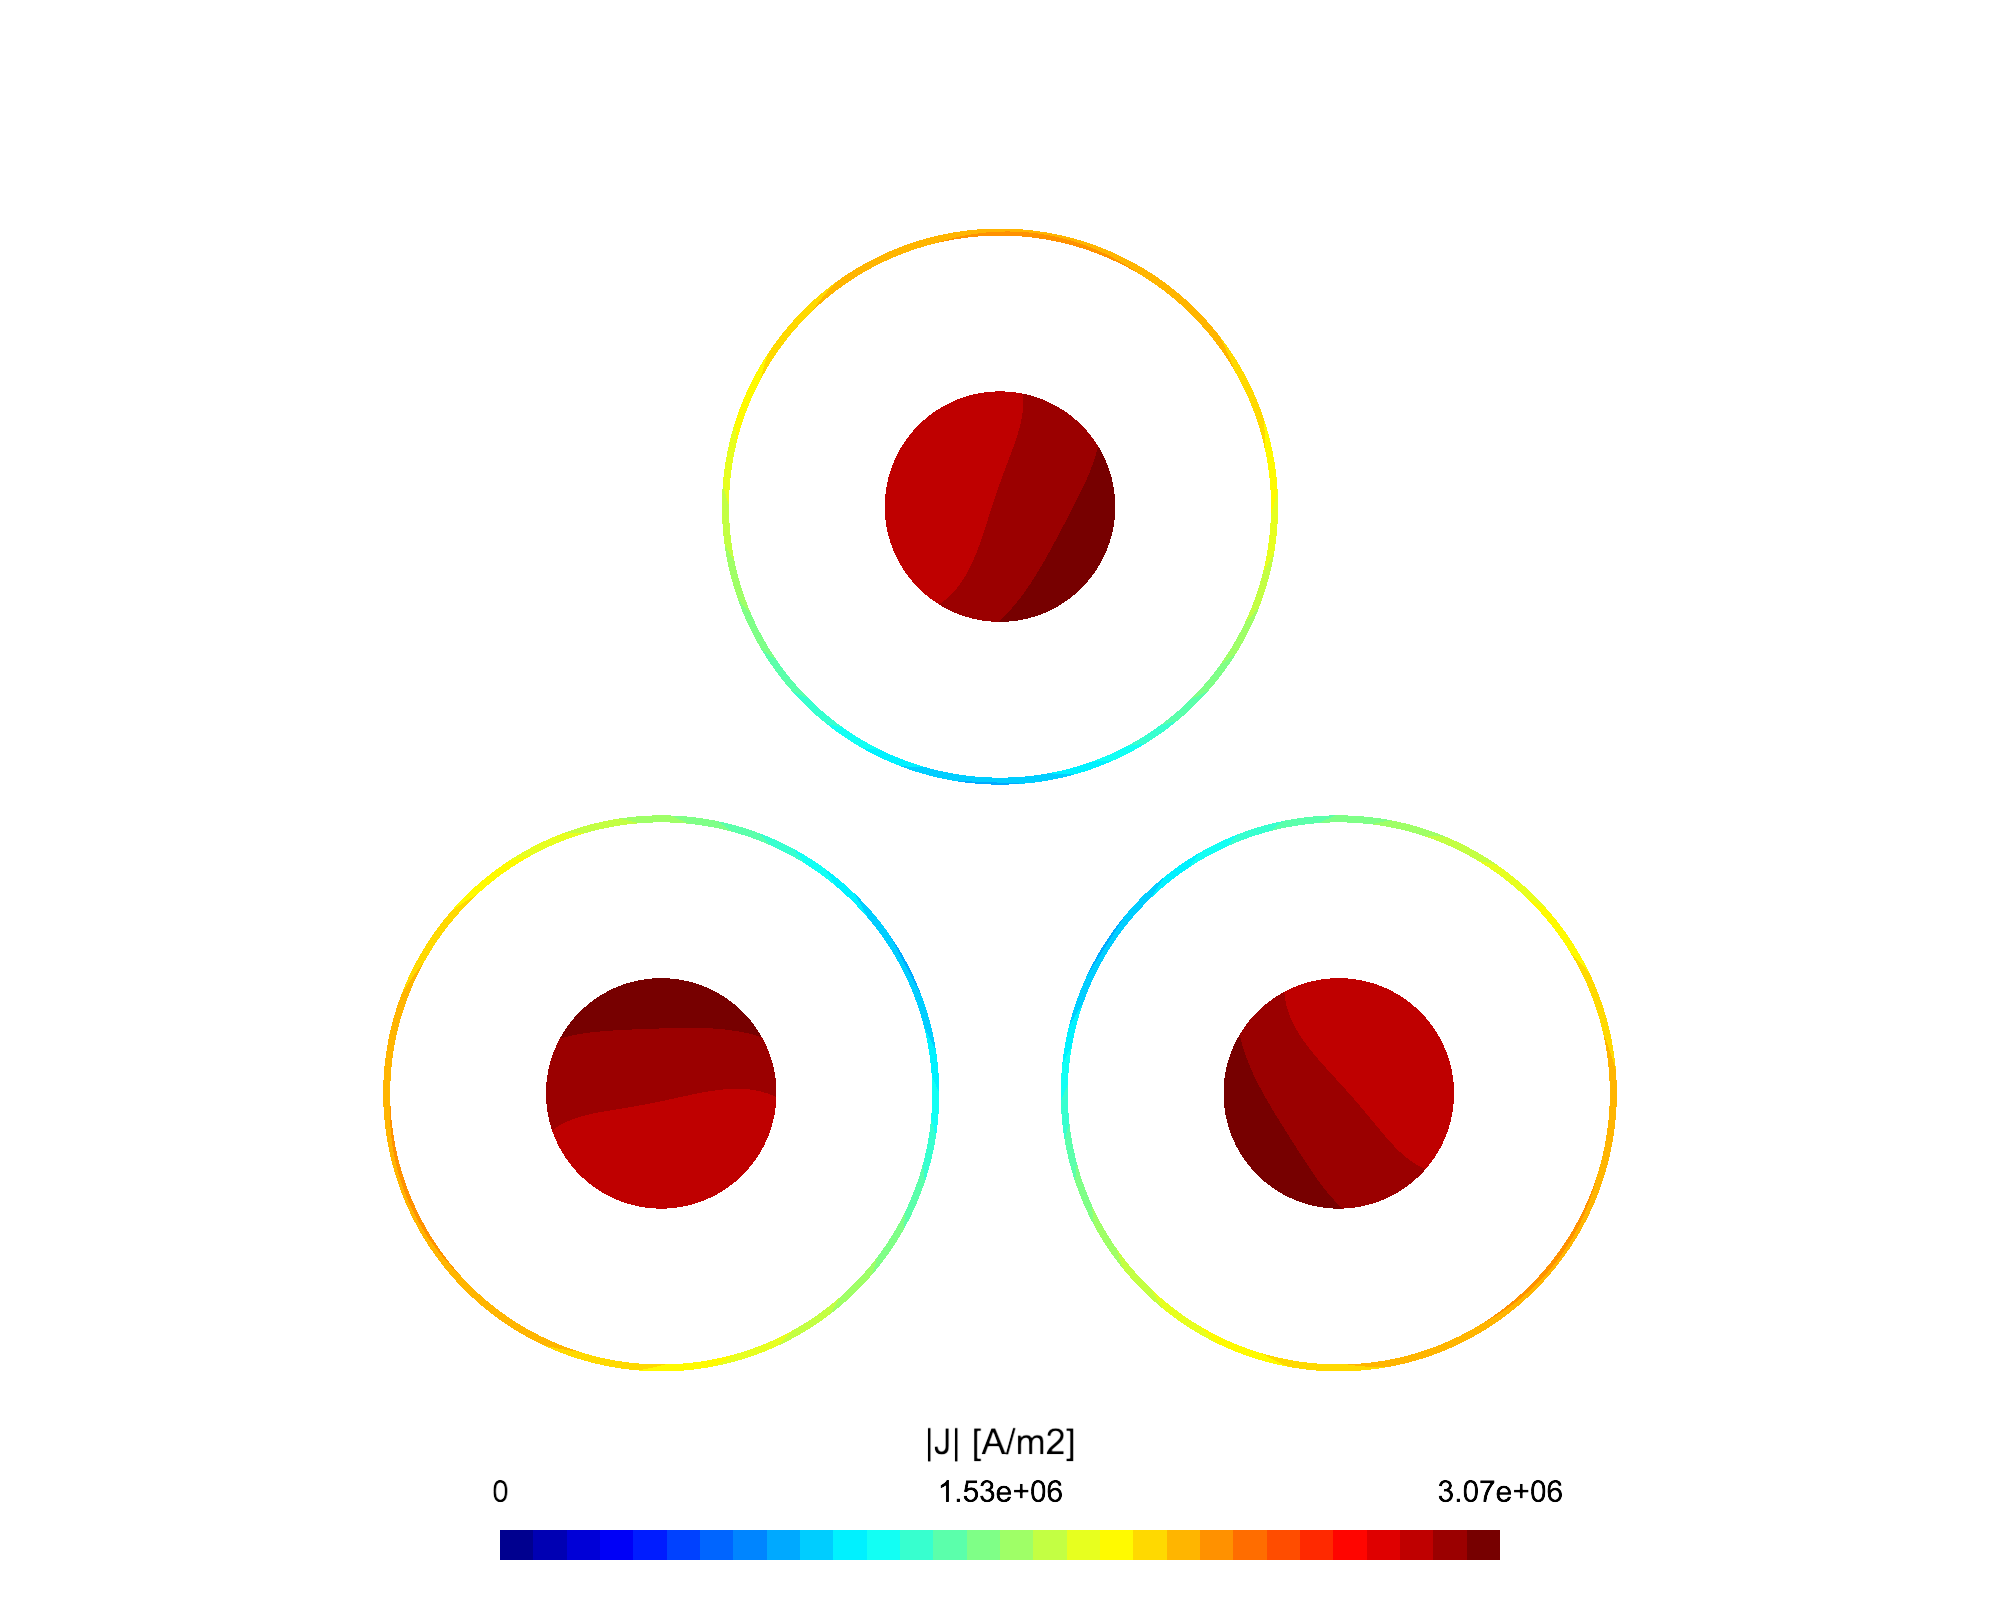
\includegraphics[width=0.23\linewidth,trim=150 0 150 0,clip]{m_j.png}\hfill
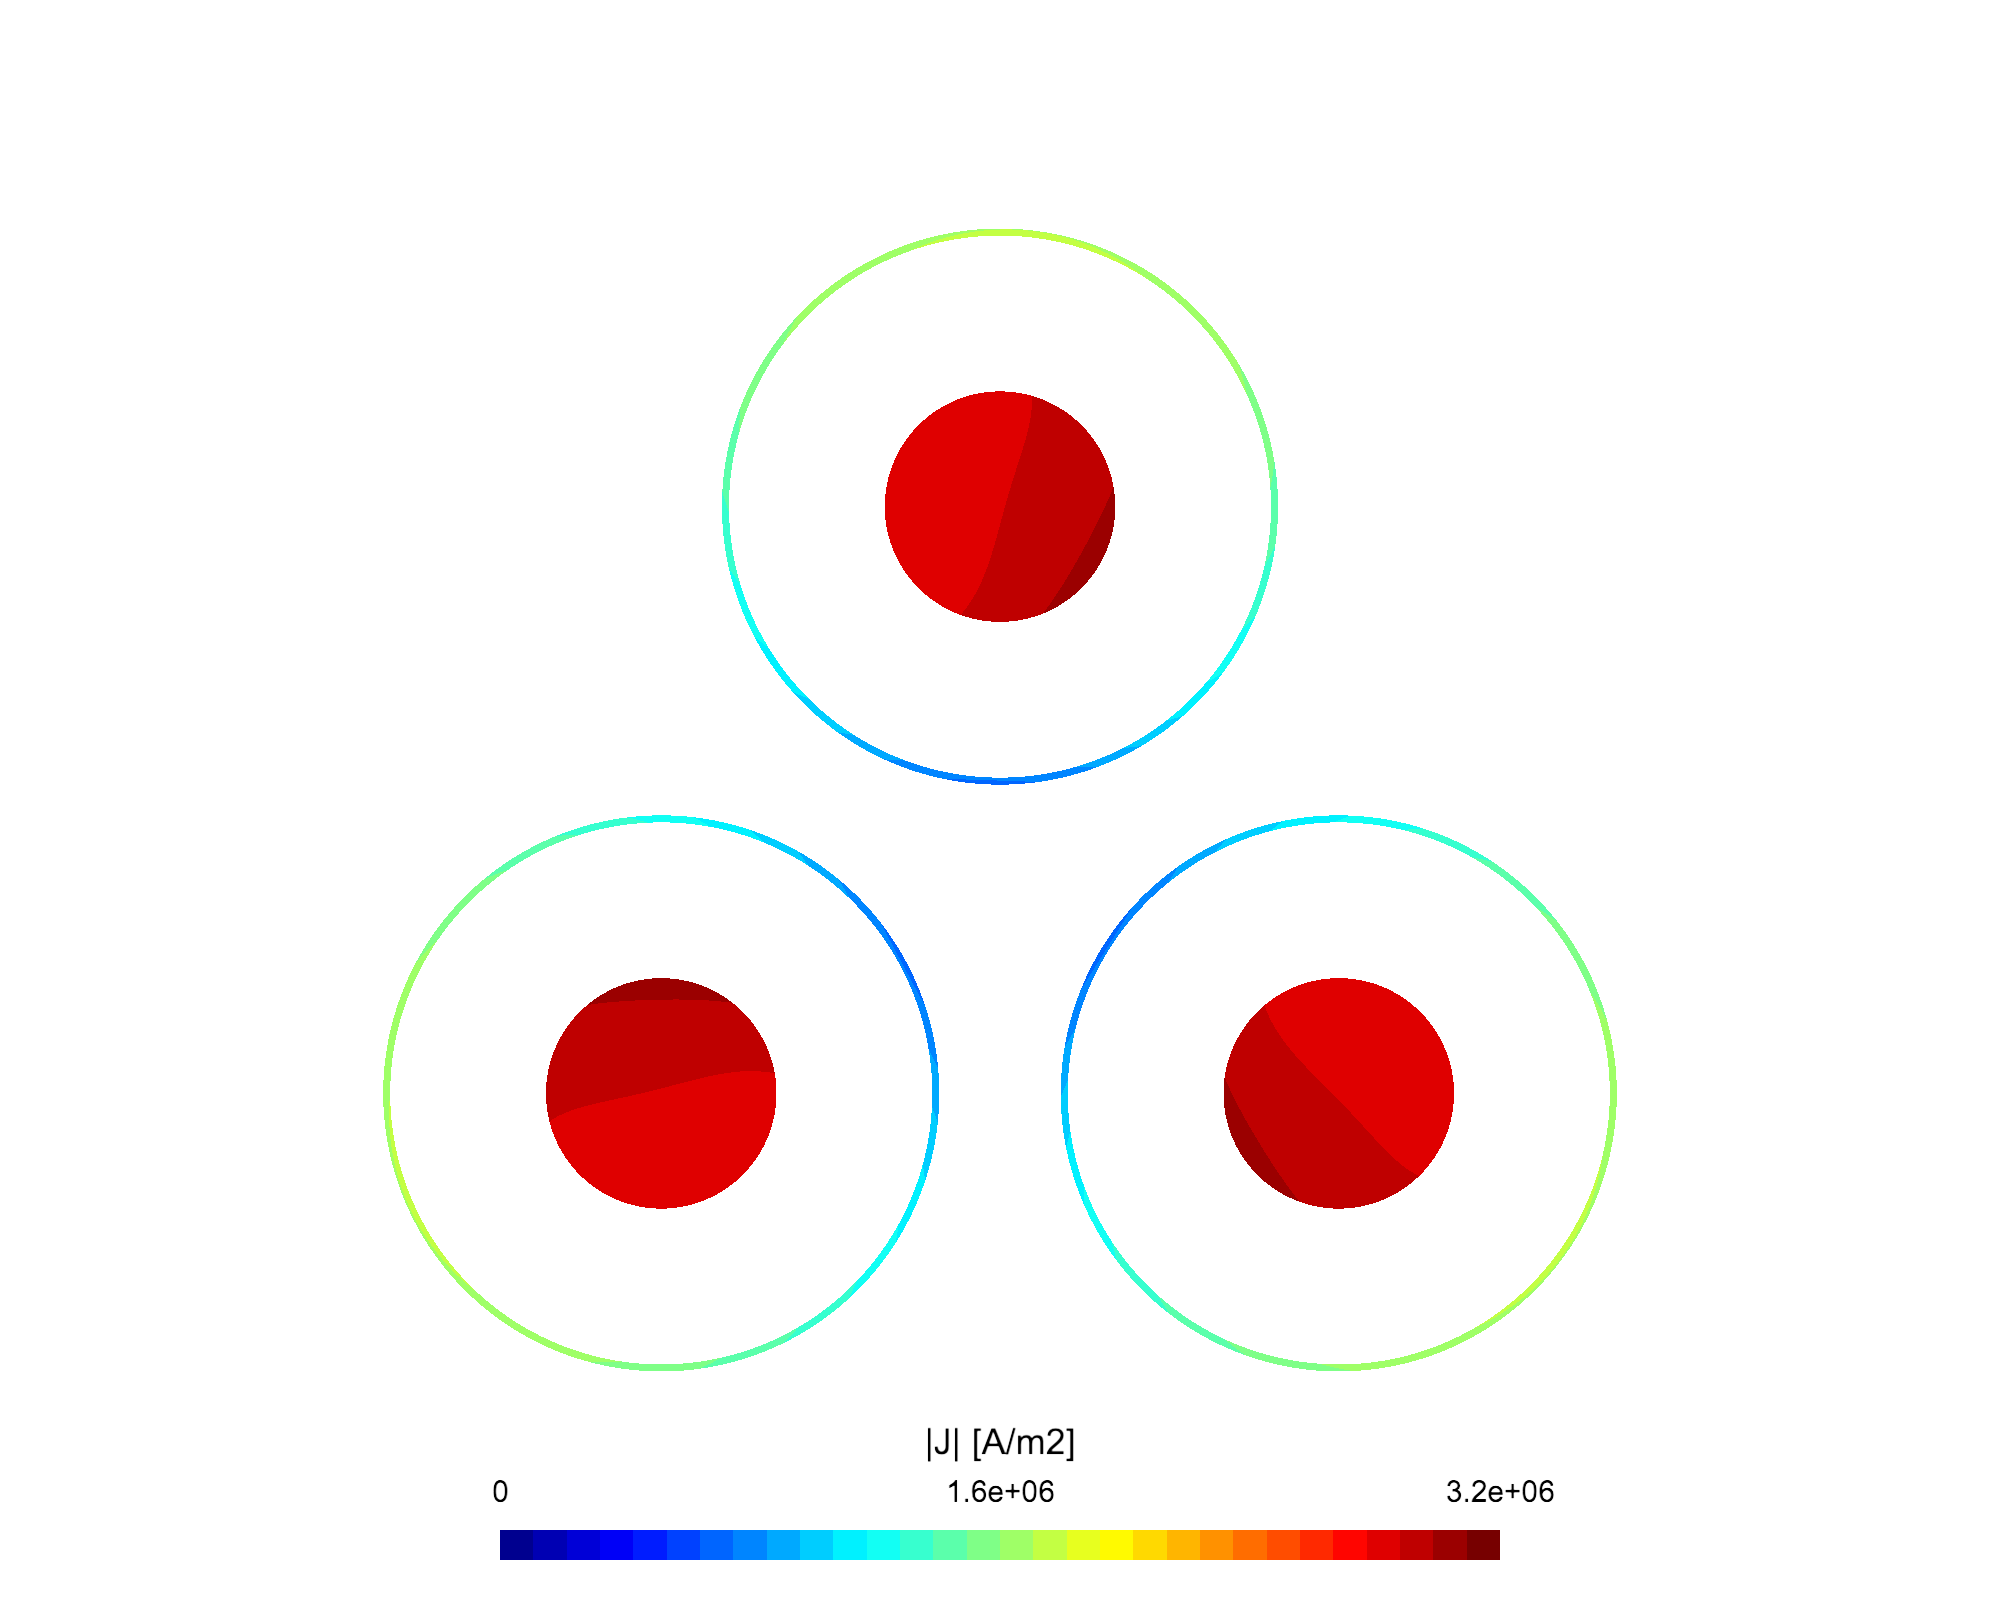
\includegraphics[width=0.23\linewidth,trim=150 0 150 0,clip]{m_j_nl.png}\\
{\small \(|\hat{\mathbf B}|\) linear / \(\sigma(T)\), then \(|\hat{\mathbf J}|\) linear / \(\sigma(T)\) (same colour scales).
Temperature maps: Q4.4.}\end{center}

\codeguide{\tfile: \texttt{Flag\_NL}.}{Gmsh: \textbf{Thermal > Conductivity model} = Linear, \textbf{Run}; then the default \(\sigma(T)\), \textbf{Run}.
\runall: cases \texttt{lin}, \texttt{nl}.}{All \texttt{.dat} outputs.}

\section*{Q4.9 Is the linear model conservative?}
\assignmentquestion{\QuestionFourNine}
\answer{\AnsFourNine}
The linear ampacity is \(350\sqrt{75/(T_{\rm lin}-15)}\), because the temperature rise is proportional
to \(I^2\). Evaluating \(\sigma\) at 90\,\(^\circ\)C is conservative for the conductor but not for the
screen losses (Q4.8).

\begin{center}\def\figw{0.75\linewidth}\def\figh{5.2cm}% Shared pgfplots style for the report and the slides. \figw / \figh set the size.
\providecommand{\figw}{0.95\linewidth}\providecommand{\figh}{5.2cm}
\providecommand{\datadir}{data}
\ifdefined\figwlen\else\newlength\figwlen\fi\setlength{\figwlen}{\figw}
\pgfplotsset{every axis/.append style={width=\figw,height=\figh,grid=major,
  grid style={gray!25},tick label style={font=\scriptsize},label style={font=\small},
  legend style={font=\scriptsize,draw=none,fill=white,fill opacity=0.85,text opacity=1}}}
\definecolor{cA}{HTML}{254C58}\definecolor{cB}{HTML}{D1495B}\definecolor{cC}{HTML}{EDAE49}
% Q4.9: hot spot versus current. Linear model: T - 15 grows exactly with I^2. sigma(T): straight in
% I^2 through the coupled solutions at 350 A (Section 4) and at the FE ampacity (90 C, Section 5).
\begin{tikzpicture}\begin{axis}[xlabel={Phase current [A RMS]},ylabel={$T_{\max}$ [$^\circ$C]},xmin=300,xmax=400,
  ymin=55,ymax=105,samples=40,
  legend style={at={(0.5,1.03)},anchor=south,legend columns=-1,/tikz/every even column/.append style={column sep=6pt}}]
\addplot[cA,thick,domain=300:400] {15+(\Tclin-15)*(x/350)^2};
\addplot[cB,thick,domain=320:380] {\Tcnl+(x^2-350^2)*(90-\Tcnl)/(\Amptrefoil^2-350^2)};
\addplot[black,dashed,domain=300:400] {90};
\addplot[cA,densely dotted] coordinates {(\AmpLin,55) (\AmpLin,90)};
\addplot[cB,densely dotted] coordinates {(\Amptrefoil,55) (\Amptrefoil,90)};
\legend{linear,\(\sigma(T)\),90\,\(^\circ\)C limit}
\node[anchor=south west,font=\scriptsize,cA] at (axis cs:\AmpLin,56) {\AmpLin\ A};
\node[anchor=south east,font=\scriptsize,cB] at (axis cs:\Amptrefoil,56) {\Amptrefoil\ A};
\end{axis}\end{tikzpicture}

\figcap{Hot spot versus current. The linear model reaches 90\,\(^\circ\)C only at \AmpLin\ A; with \(\sigma(T)\)
the limit is reached at \Amptrefoil\ A (straight line in \(I^2\) through the coupled solutions at 350 A and at
the FE ampacity of Section 5).}\end{center}
\subsection*{Sources}
\small \textbf{[Lienhard]} J.H.~Lienhard~V, J.H.~Lienhard~IV, \refurl{https://ahtt.mit.edu/}{\emph{A Heat Transfer Textbook}}, 6th ed., v6.00 (2024), free PDF: eq.~(8.35), p.~435 (hot horizontal plate facing up, \(\mathrm{Nu}=0.14\,\mathrm{Ra}^{1/3}\)) and eq.~(2.31), p.~72 (\(h_{\rm rad}=4\sigma T_m^3\varepsilon\)).
\textbf{[KTH]} L.~Lindstr\"om, \refurl{https://www.diva-portal.org/smash/get/diva2:511556/fulltext01.pdf}{\emph{Evaluating impact on ampacity according to IEC-60287 regarding thermally unfavourable placement of power cables}}, MSc thesis, KTH Stockholm (2011): IEC 60287 equations, eqs.~(4.1)--(4.2) (ladder, ampacity), (4.6)--(4.14) (\(y_s,y_p,\lambda_1\), \(W_d\)), (4.17) (\(T_3\)).
\textbf{[UNCC]} A.A.~Nche, \refurl{https://ninercommons.charlotte.edu/record/695/files/AkumawahNche_uncc_0694N_11459.pdf}{\emph{Temperature modeling and control algorithm for high voltage underground cables}}, MSc thesis, Univ.\ of North Carolina at Charlotte (2017), eq.~(19), p.~21 (\(T_1=\frac{\rho}{2\pi}\ln(D_{oi}/d_c)\)).
\textbf{[Karlstrand]} J.~Karlstrand, M.~Hatlo, M.~Hovde, \refurl{https://jicable.org/TOUT_JICABLE_FIRST_PAGE/2023/2023-P3-5_page1.pdf}{``Evaluation of thermal resistances \(T_3\) and \(T_4\) for touching formations in IEC 60287-2-1''}, Jicable'23, paper P3-5, eq.~[2]: \(T_4=\frac{n\rho}{2\pi}[\ln(2u)-\delta]\), touching trefoil \(n=3\), \(\delta=0.630\) (free first page).
\textbf{[Jicable]} M.~El~Chmouri, \refurl{https://jicable.org/TOUT_JICABLE_FIRST_PAGE/2023/2023-E10-4_page1.pdf}{``Influence of the dielectric losses in EHV cables on the cable temperature during laboratory testing''}, Jicable'23, paper E10-4, Table 1: IEC 60287-1-1 dielectric loss needed for unfilled XLPE only from \(U_0=127\) kV (free first page).
[\v{S}u\'{c}urovi\'{c}] (\(\tan\delta\)) and [Enescu] (\(\rho_T=3.5\) K\,m/W): Section 1.
Local \href{../NMES_Assignment_2026.pdf}{assignment} (eqs.\ 10--12, 15) and
\href{../Datasheet NKT 33 kV single core cable XLPE-AL.pdf}{NKT datasheet} (rating conditions).
\end{document}
